\hypertarget{introduction}{%
\section{Introduction}\label{introduction1}}

To generate three-dimensional epithelial structures in vitro from planar epithelial monolayers, we chose to utilize an existing system of epithelial domes (spontaneous domes) developed by Ernest Latorre and improved by Ariadna Marin-Llauradó  \cite{latorre2018,marin-llaurado2022}. This system involves seeding a Madin-Darby canine kidney (MDCK) cell monolayer on a substrate that is patterned with circular non-adhesive regions. The cells invade these regions and form a cohesive monolayer everywhere within 24 to 48 hours. Due to the active ion pumping mechanism of the MDCK cells in the apical-to-basal direction, the cells delaminate from impermeable substrates such as glass or soft PDMS gel and form spherical cap structures on the circular patterns, known as epithelial domes. Latorre and Marin-Llauradó demonstrated that they could form a variety of structures with controlled shape and size, ranging from spherical to tubular caps.  

This system also enables the use of 3D traction force microscopy to measure pressure. The technique involves measuring the deformation of a soft PDMS gel embedded with beads to characterize the forces and pressures applied by the cells on the substrate. This method offers an innovative approach to measuring pressure compared to the previous technique of puncturing epithelial domes with a microneedle \cite{tanner1983, choudhury2022}. It also allows for the characterization of the rheology of epithelia and the discovery of interesting material properties such as the superelasticity of cells during stretching \cite{latorre2018}.  

However, the formation of epithelial domes is dependent on the ion pumping mechanism of the domes, making them spontaneous structures. Therefore, the timescales for the dome stretching are not controlled, although this process can be marginally accelerated by a few hours through the use of drugs like Forskolin, which can activate transepithelial channels of NA+/K+/Cl- \cite{klebe1995,bourke1987}. Furthermore, not all epithelial tissues actively pump ions or do it with the required polarity for dome formation. In this chapter, we will be discussing a microfluidic chip that can inflate an epithelial monolayer into a dome with arbitrary time evolution of applied pressure while also allowing us to measure and control the forces involved.


\hypertarget{monolayer-inflator}{%
\section{Monolayer Inflator}\label{monolayer-inflator}}

\begin{figure}[b!]
	\centering
	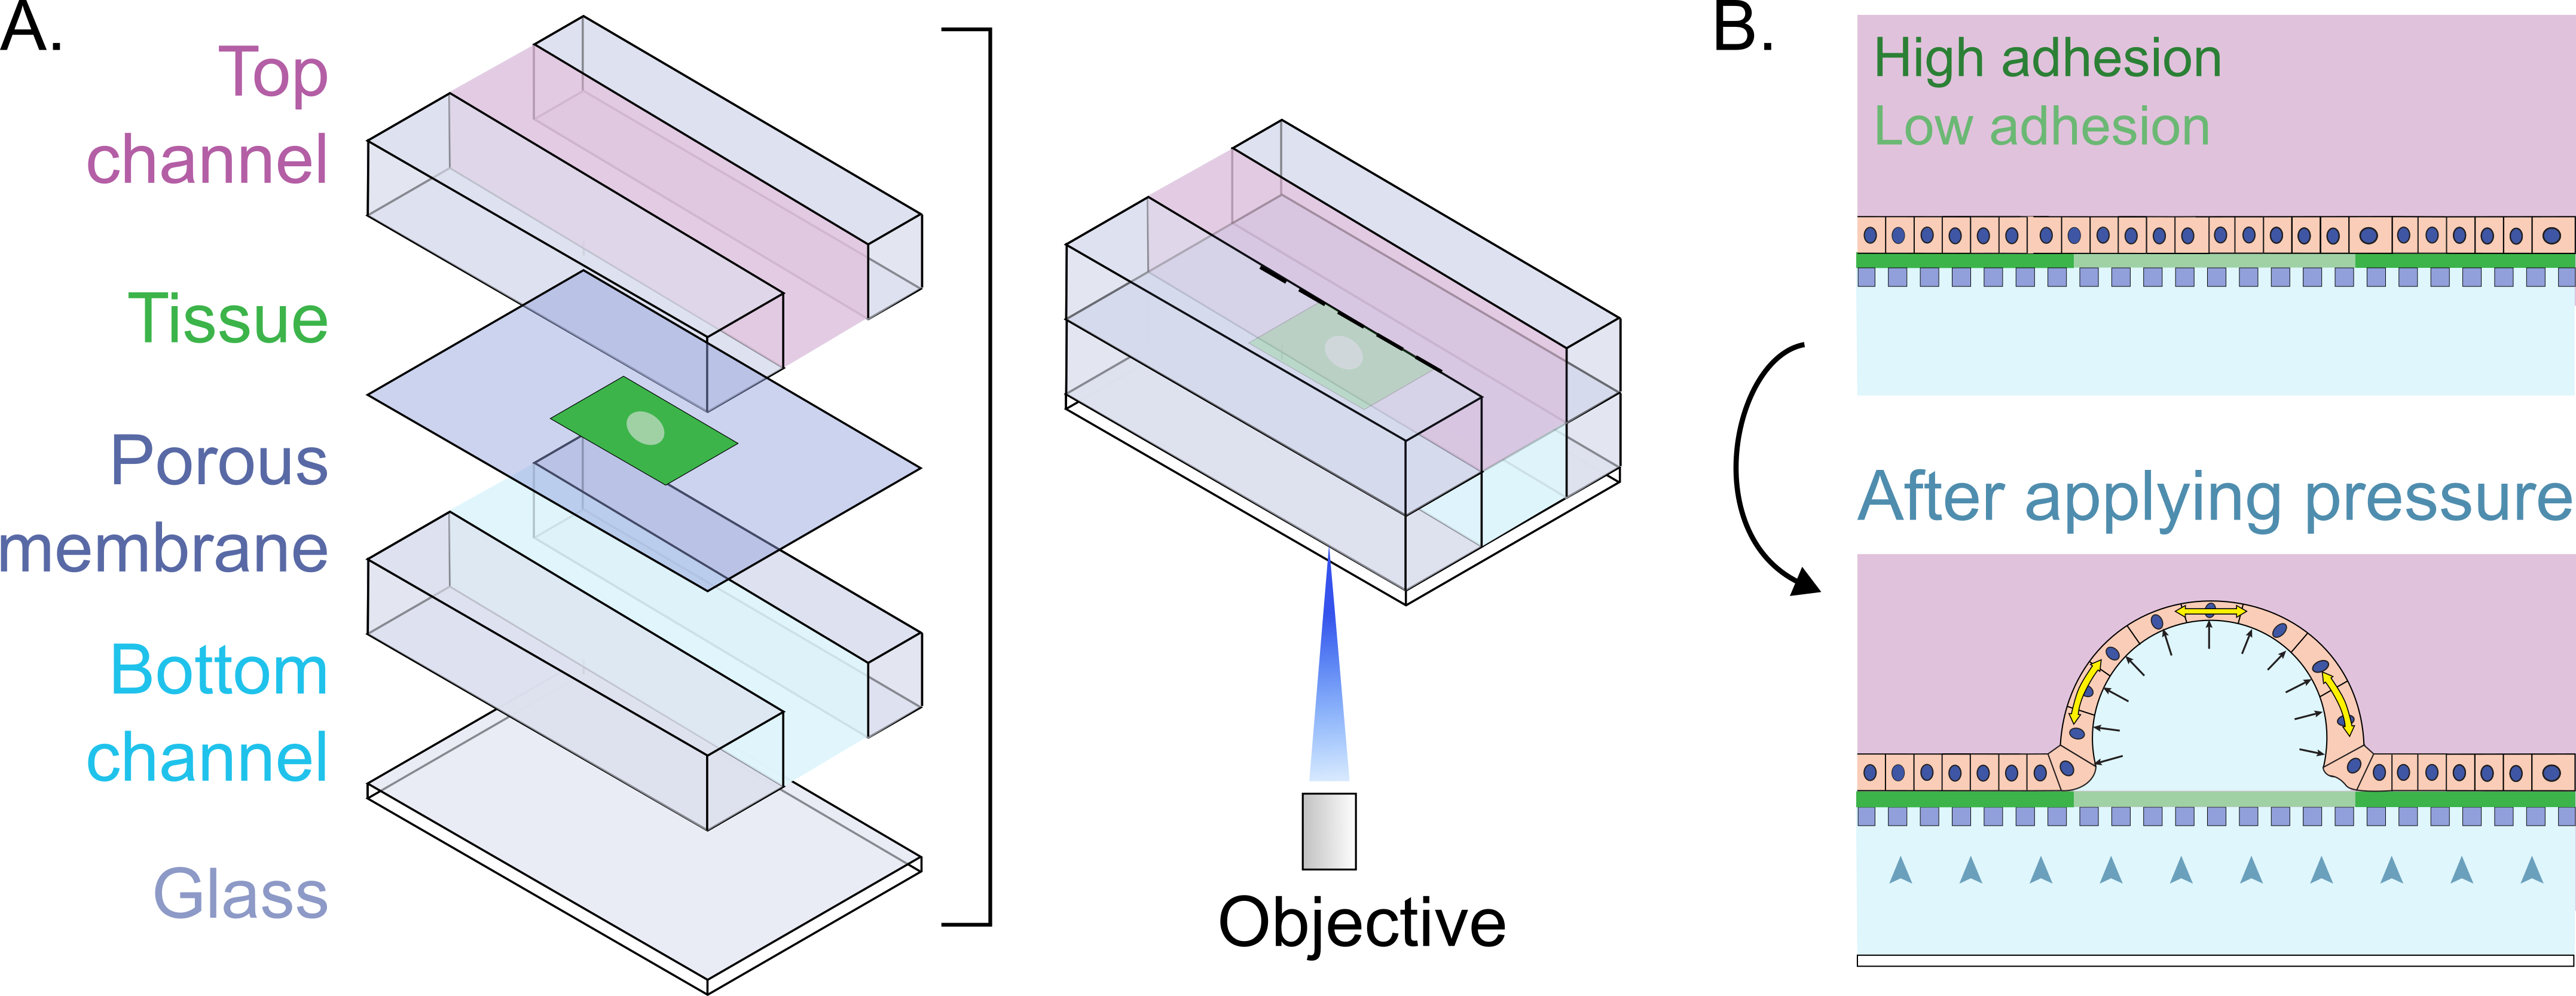
\includegraphics[width=\textwidth]{chap6_scheme.png}
	\caption{\textbf{Conceptual design of MOLI}: (A) Microfluidic device consist of a porous membrane sandwiched between two layers of schannels. (B) Upon application of pressure, cells from low adhesion will detach to form an epithelial dome. 
	}\label{fig_6_1}
\end{figure}

Drawing inspiration from the pioneering work on organ-on-chip microfluidic devices, we have deemed these platforms to be an ideal system for the precise manipulation of pressure, cell culture conditions, and the acquisition of high-resolution imaging data \cite{huh2010, nelson2017}. An illustrative example is the lungs-on-chip device, which comprises two distinct layers separated by a porous membrane. The top layer contains a channel for the epithelial cells, while the bottom layer has a channel for the endothelial cells. This device is assembled on a thin glass slide, which facilitates the collection of high-quality imaging data. 

Therefore, we conceived the idea of a MOnoLayer Inflator (MOLI) device, which utilizes a two-layer microfluidic channel with one side for epithelial monolayers and the other for the application of pressure (see Fig. \ref{fig_6_1}). The epithelial monolayer side is micropatterned with a protein that contains non-adhesive or less-adhesive regions for dome formation. Our working hypothesis postulated that cells would adhere to the protein substrate uniformly, even in regions with lower adhesive properties. We anticipated that upon the application of pressure, cells would detach from the regions with weaker adhesion, leading to the formation of a dome-shaped structure.

We attempted to fabricate the devices by utilizing plastic stickers and photopolymerizable adhesive, but encountered difficulties such as fluid leakage and limited biocompatibility, rendering them unsuitable \cite{sollier2011, bartolo2008}. Consequently, we opted for the utilization of PDMS material to construct the microfluidic chip due to its facile handling and processing characteristics.


\hypertarget{fabrication-of-the-device}{%
\section{Fabrication of the device}\label{fabrication-of-the-device}}

\begin{figure}[b!]
	\centering
	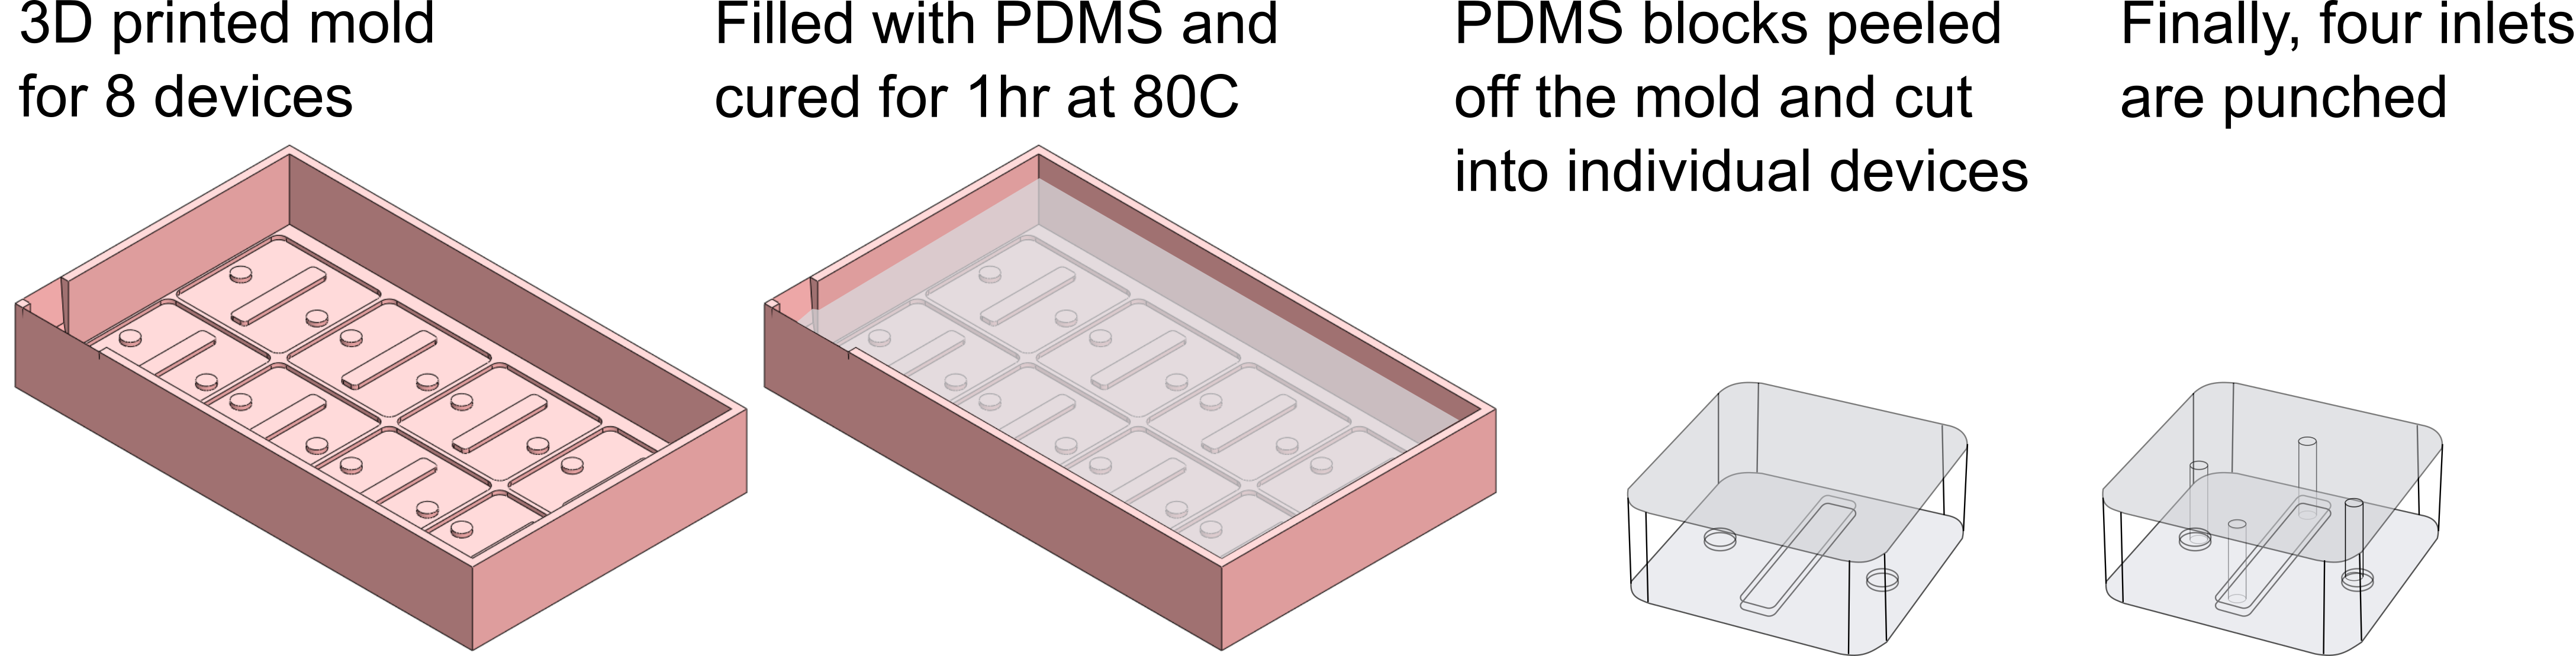
\includegraphics[width=\textwidth]{chap6_mold.png}
	\caption{ \textbf{3D printed mold for the device} patterned to prepare eight devices at a time. The thickness of the PDMS block is controlled with volume of PDMS poured into the mold. After polymerization, the PDMS is cut into individual pieces and inlets are punched with a biopsy punch.}\label{fig_6_1a}
\end{figure}

The structure of the device consists of four layers: glass, bottom channel, porous membrane, and top channel. These layers are bonded together using ozone plasma activation.

For imaging epithelial structures with high-resolution confocal microscopy, the device must be mounted on a thin glass slide. We used \#0 glass slides, which have a thickness range of 85-115 \unit{\um} and are designed for high-performance microscopy applications. 

To ensure that the porous membrane is positioned as close as possible to the microscope objectives, whose working distance typically ranges between 200\unit{\um} and 1000\unit{\um}, it is crucial that the channel is sufficiently thin. To this end, we fabricated the bottom layer with a thickness of 100\unit{\um}. This thickness provides adequate structural support for manual handling, while avoiding potential microfluidic issues arising from pressure loss and lower flow rates. To achieve the desired thickness, we utilized a spin coating method to fabricate a thin layer of polydimethylsiloxane (PDMS). Subsequently, the layer was precisely cut into the channel shape using a desktop cutting machine (Silhouette Cameo 4, Silhouette America).

The primary function of the porous membrane is to enable pressure application while preventing the migration of cells from the cell channel to the pressure channel. Initially, we used a membrane with pores of 10\unit{\um} diameter based on literature. We attempted to create 10\unit{\um} pores in a 100\unit{\um} thin layer of PDMS using photolithography to facilitate manual handling. However, we encountered difficulty in fabricating 10\unit{\um} pillars with a height of 100\unit{\um} due to an excessively high aspect ratio, making the pillars too fragile and prone to breakage during fabrication. Therefore, we opted to employ plastic, polyethylene terephthalate (PET), membranes with 10\unit{\um} pores. 

\begin{figure}[h!]
	\centering
	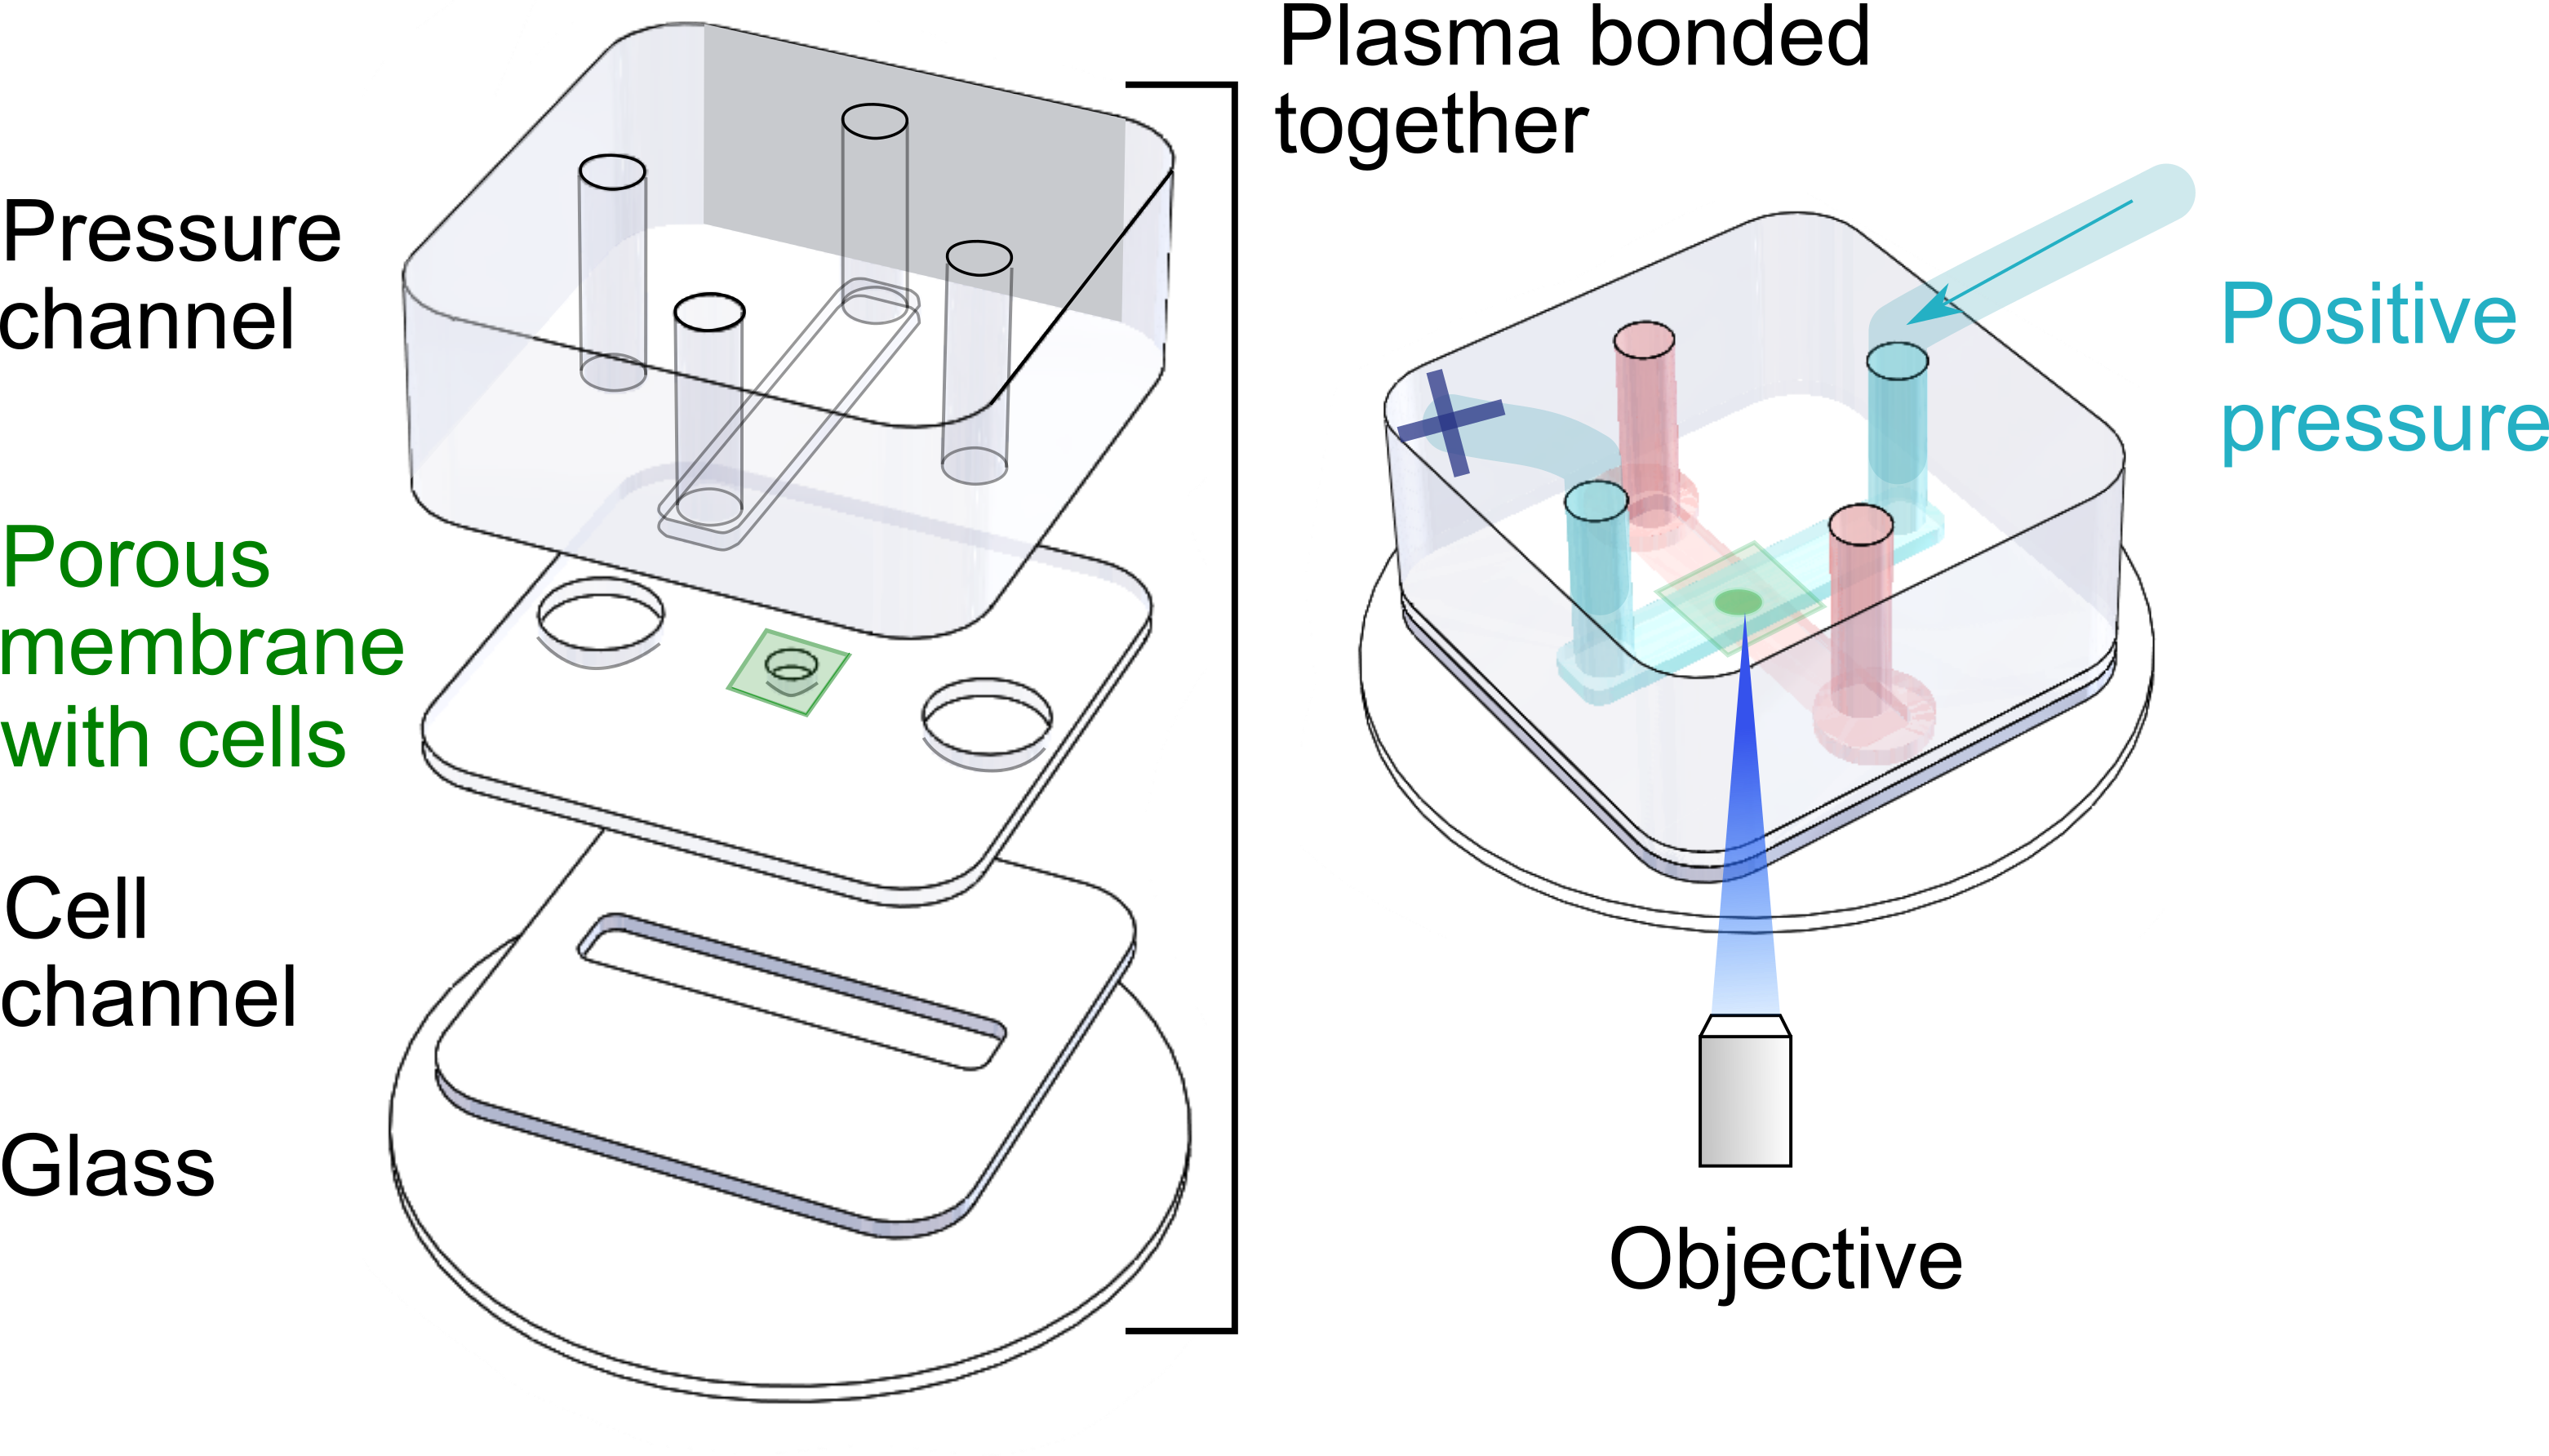
\includegraphics[width=0.75\textwidth]{chap6_realscheme.png}
	\caption{ \textbf{Fabrication of MOLI}: Four layers assembled together with ozone plasma cleaning. Each channels has a inlet and outlet. Only the pressure channel is connected to the tubing; one side connects to the reservoir and other is sealed. 
	}\label{fig_6_2}
\end{figure}

\clearpage

The thin (10\unit{\um}) plastic sheets were easily manageable, but we encountered difficulties with bonding and experienced leakages due to membrane wrinkling. To address these difficulties, we decided to modify the middle layer by using a PDMS layer with a hole attached to a small piece of membrane, instead of whole layer being a porous membrane. This approach allowed us to achieve stronger and leak-proof bonding by sandwiching a smaller area between the two PDMS layers. The middle PDMS thin layer was constructed with a 1.2\unit{\mm} hole to expose the membrane to pressure, as this dimension is approximately the size of the field of view of a 10X objective.

The design of the top channel in the device involved a PDMS block with a 5\unit{\mm} thickness and a 1mm engraved channel. The decision to select the thickness of the top channel was based on the requirement for the block to be sufficiently thick to accommodate tubing for pressure application.  To create the mold with the channel, a precision 3D printer (Solus DLP 3D Printer) was utilized. Additionally, four inlets with a diameter of 1.5\unit{\mm} were punched into the block using a biopsy punch to facilitate two inlets for the pressure channel and two inlets for cell seeding purposes  (see Fig.~\ref{fig_6_1a}).

Ultimately, the integration of the layers was accomplished through a two-step bonding process utilizing an ozone plasma cleaner (refer to Fig. \ref{fig_6_2}). First, we bonded the glass to the bottom channel and simultaneously bonded the middle layer to the top channel. Following this step, the two assembled layers were bonded together with the membrane sandwiched in the middle to create the final device.
\vspace{-0.05cm}
\hypertarget{protein-patterning-and-inverted-cell-culture}{%
\section{Protein patterning and "upside-down" cell
culture}\label{protein-patterning-and-inverted-cell-culture}}

To overcome issues encountered in earlier prototypes, we opted to employ a glass-bottomed dish (35\unit{\mm}, \#0 coverslip thickness, Cellvis) as the container for our experimental setup. This design choice was made to address concerns surrounding the potential for cell culture medium to spill over/under the device during pressure application, especially in the case of a leaky device. 

In the context of the spontaneous dome system, the upper surface is accessible for various treatments and microcontact printing using a PDMS block. However, in our case, we have a completely sealed device, which necessitated the use of the photopatterning technique known as PRIMO. In brief, first the surface to be micropatterned is coated with poly-L-lysine (PLL) and then SVA-PEG chains. Upon illumination with UV light (375\unit{\nm}), PEG chains in selective regions could be cleaved and subsequently exposed to adhesion-promoting proteins. The PRIMO technique had been optimized previously for substrates made of glass and soft PDMS. We had to optimize the technique for use with a porous plastic membrane, which entailed increasing laser power to 1500\unit{mJ/\mm^2} (for details see the Appendix A). We also optimized coating the devices with fibronectin, vitronectin and collagen. For the experiments featured in this thesis, we are using fibronectin mixed with fluorescent fibrinogen for finding the samples.

To ensure successful attachment of cells and formation of monolayer, a concentration of 25-30×\unit{\num{e6} cells/\ml} was seeded for one hour, followed by rigorous flushing with fresh cell culture media to wash away any unattached cells. Early experiments revealed that while cells attached to the top side of the porous membrane, there were very few dome formations upon application of pressure. Additionally, imaging through the porous membrane was poor quality, as the cells were further away from the microscope objective, and some cells were filtering through the membrane from top to bottom (see Fig. \ref{fig_6_4}).  

\begin{figure}[]
	\centering
	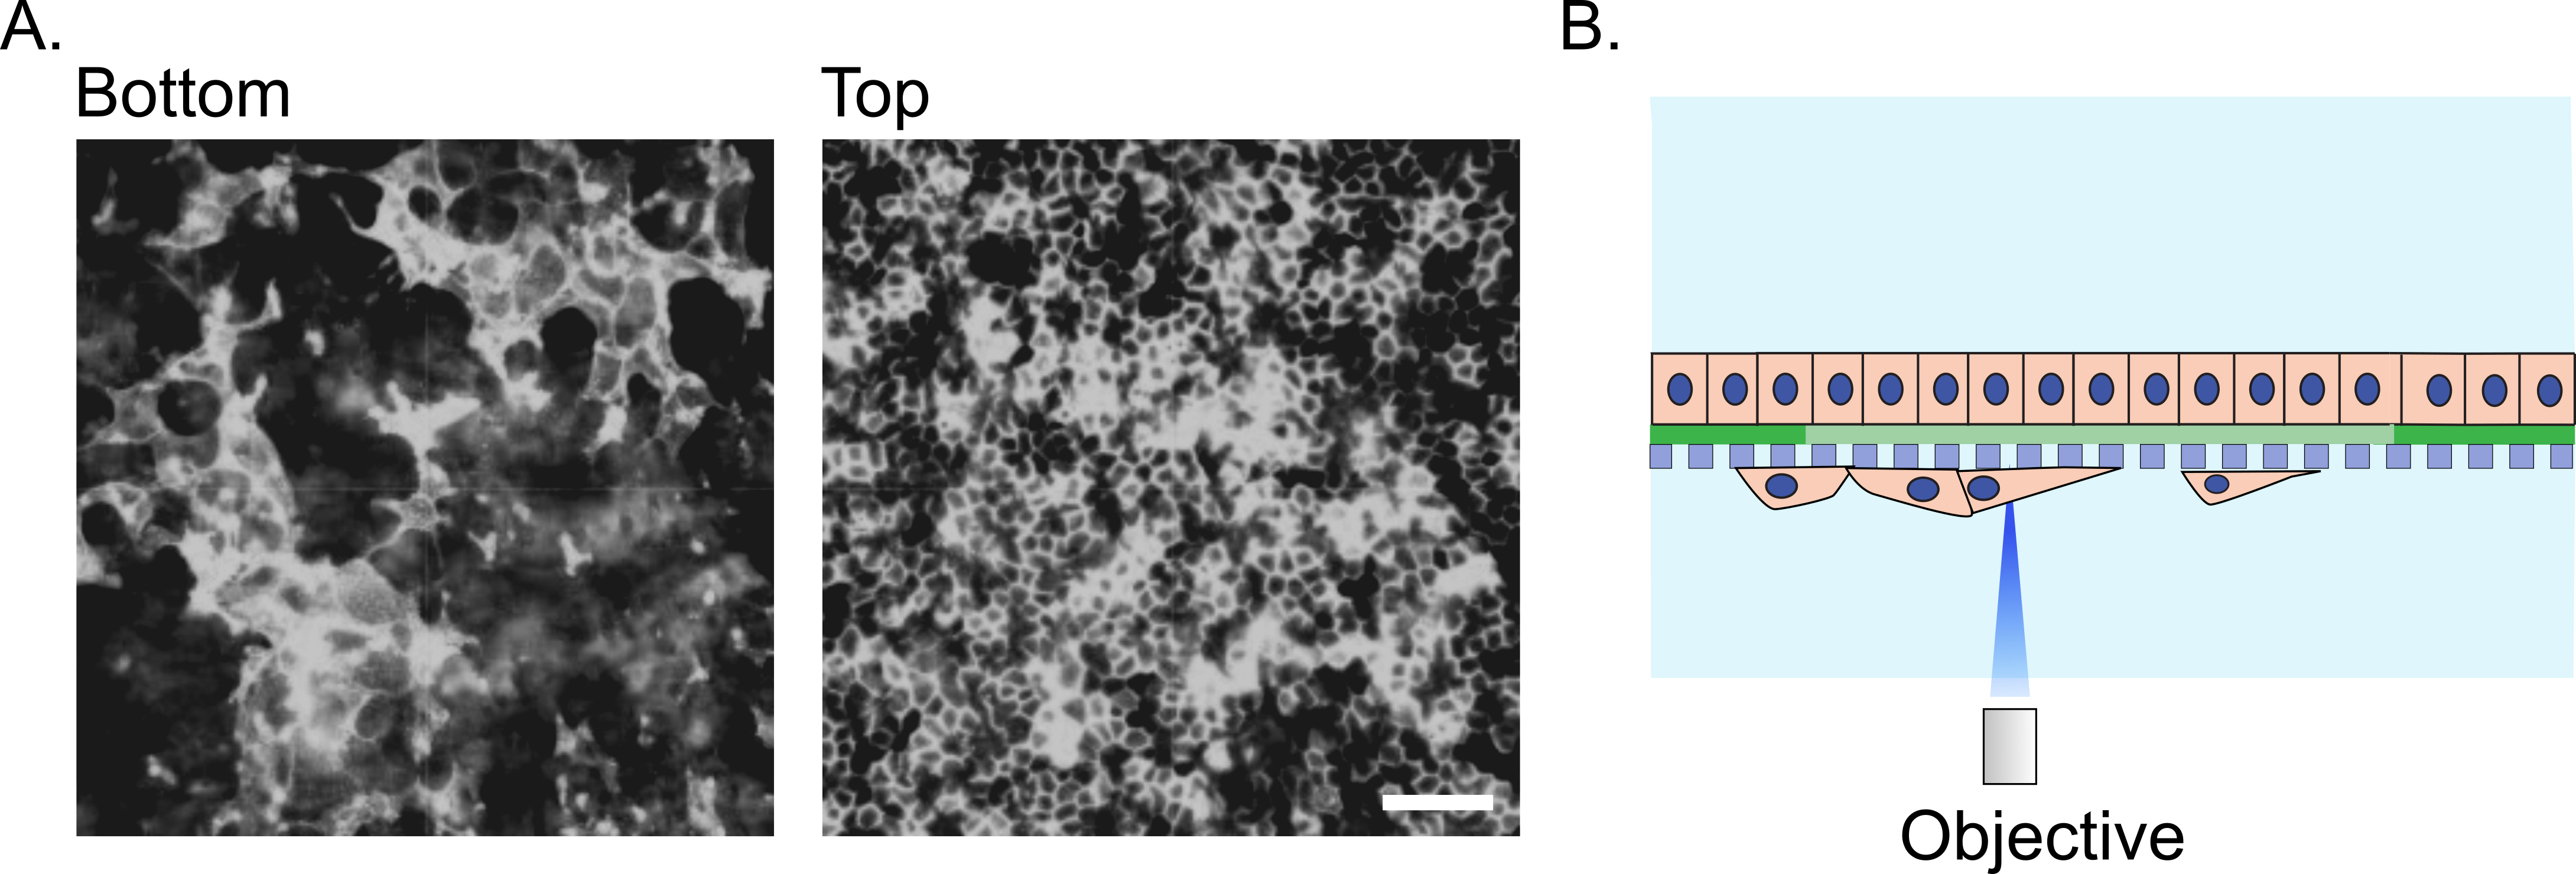
\includegraphics[width=0.75\textwidth]{chap6_cellsontop.png}
	\caption{ \textbf{Cells filtering through the membrane}: (A) Images of MDCK-CiBN CAAX GFP monolayer on the both sides of the membrane. Scale bar is $80\mu m$. (B) Schematic of imaging through the porous layer.	}\label{fig_6_4}
\end{figure}


To prevent cells from crossing the membrane, various plastic membranes with smaller pore sizes (ranging from 50 \unit{\nm} to 10 \unit{\um}) were systematically tested. Considering the flow rates and cell filtration through the membrane, a 400 \unit{\nm} pore size membrane was chosen. However, imaging the green channel (488 \unit{\nm}) through these pores was impossible. Therefore, an "upside-down" cell culture approach was implemented, where the device was flipped immediately after seeding cells in the bottom channel to ensure attachment on the membrane instead of the glass (see Fig.~\ref{fig_6_5}). Thorough washing of the channel was necessary to prevent cell attachment to the glass, which would have obstructed the imaging of the domes.

Despite optimization efforts, achieving complete coverage of non-adhesive regions with a cell monolayer remained a significant challenge. To address this issue, the protein concentration in these regions was increased to facilitate cell attachment at the designated dome location. Upon application of pressure, cells from the lower adhesion region would detach, resulting in the formation of the dome structure.

%\begin{figure}
%	\begin{minipage}[c]{0.7\textwidth}
%		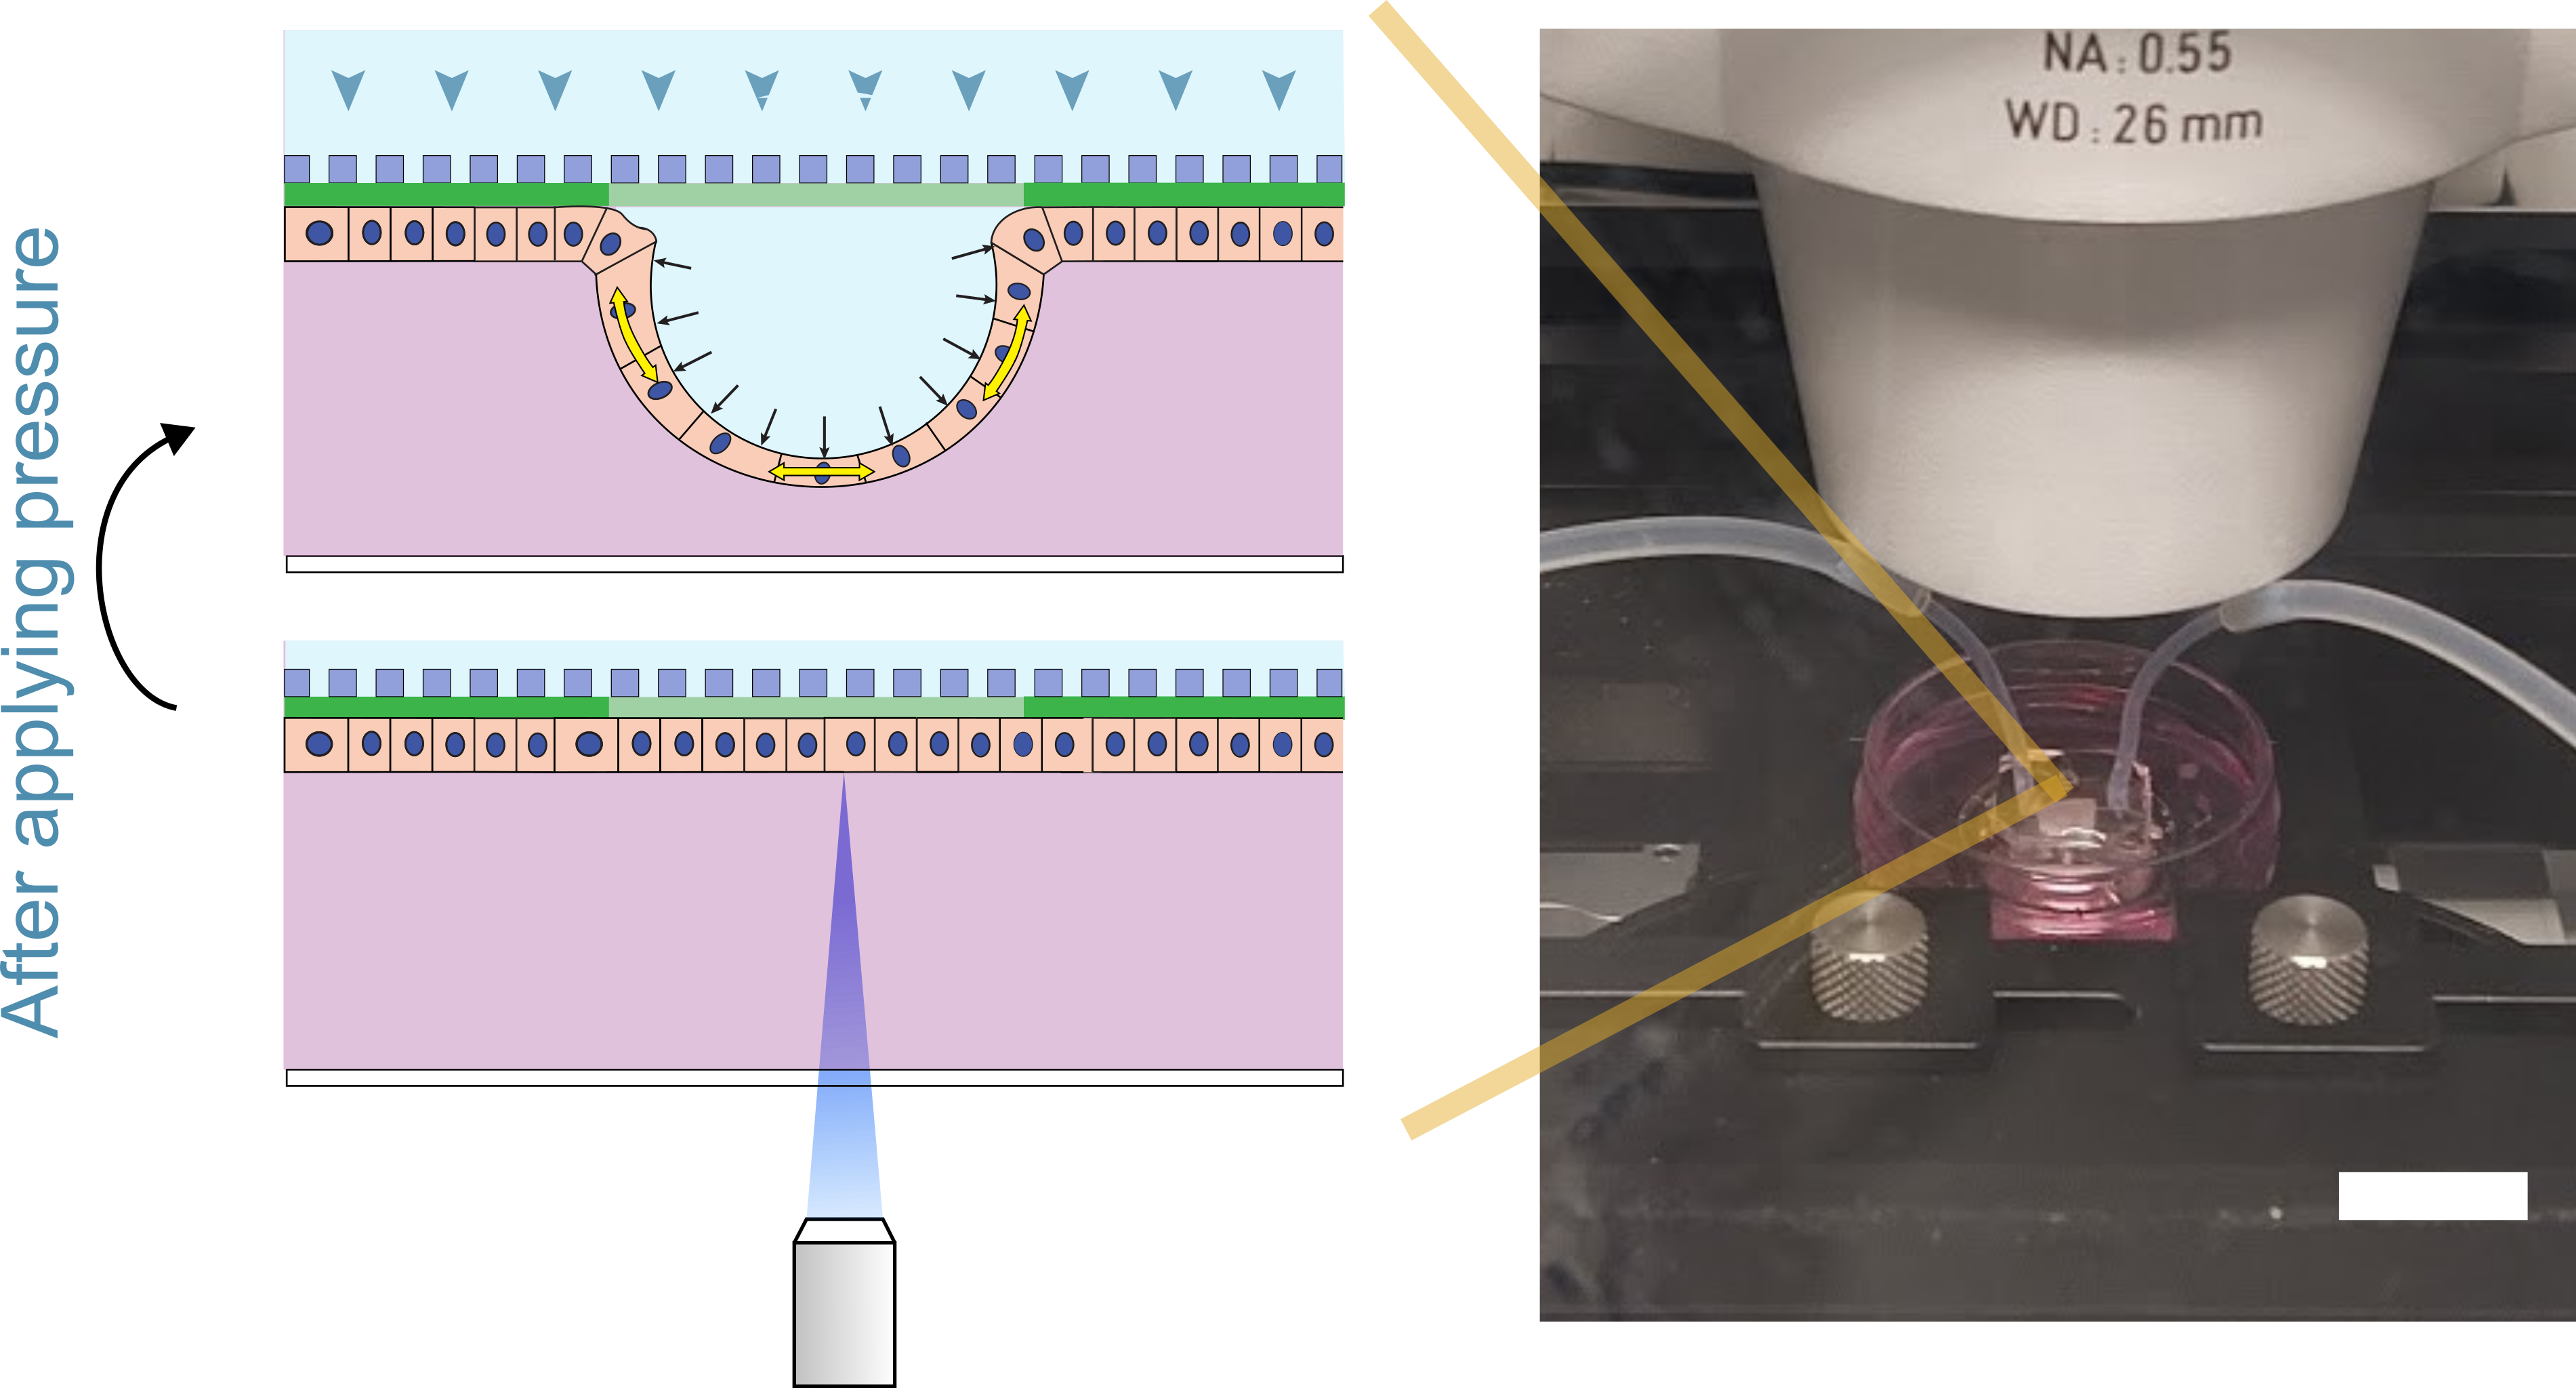
\includegraphics[width=\textwidth]{chap6_realdevice.png}
%	\end{minipage}\hfill
%	\begin{minipage}[c]{0.27\textwidth}
%		\caption{\\ \textbf{Upside-down cell culture}: Illustration of upside-down cell culture and the experimental setup on the microscope stage.
%		}\label{fig_6_5}
%	\end{minipage}
%\end{figure}

\begin{figure}[]
	\centering
	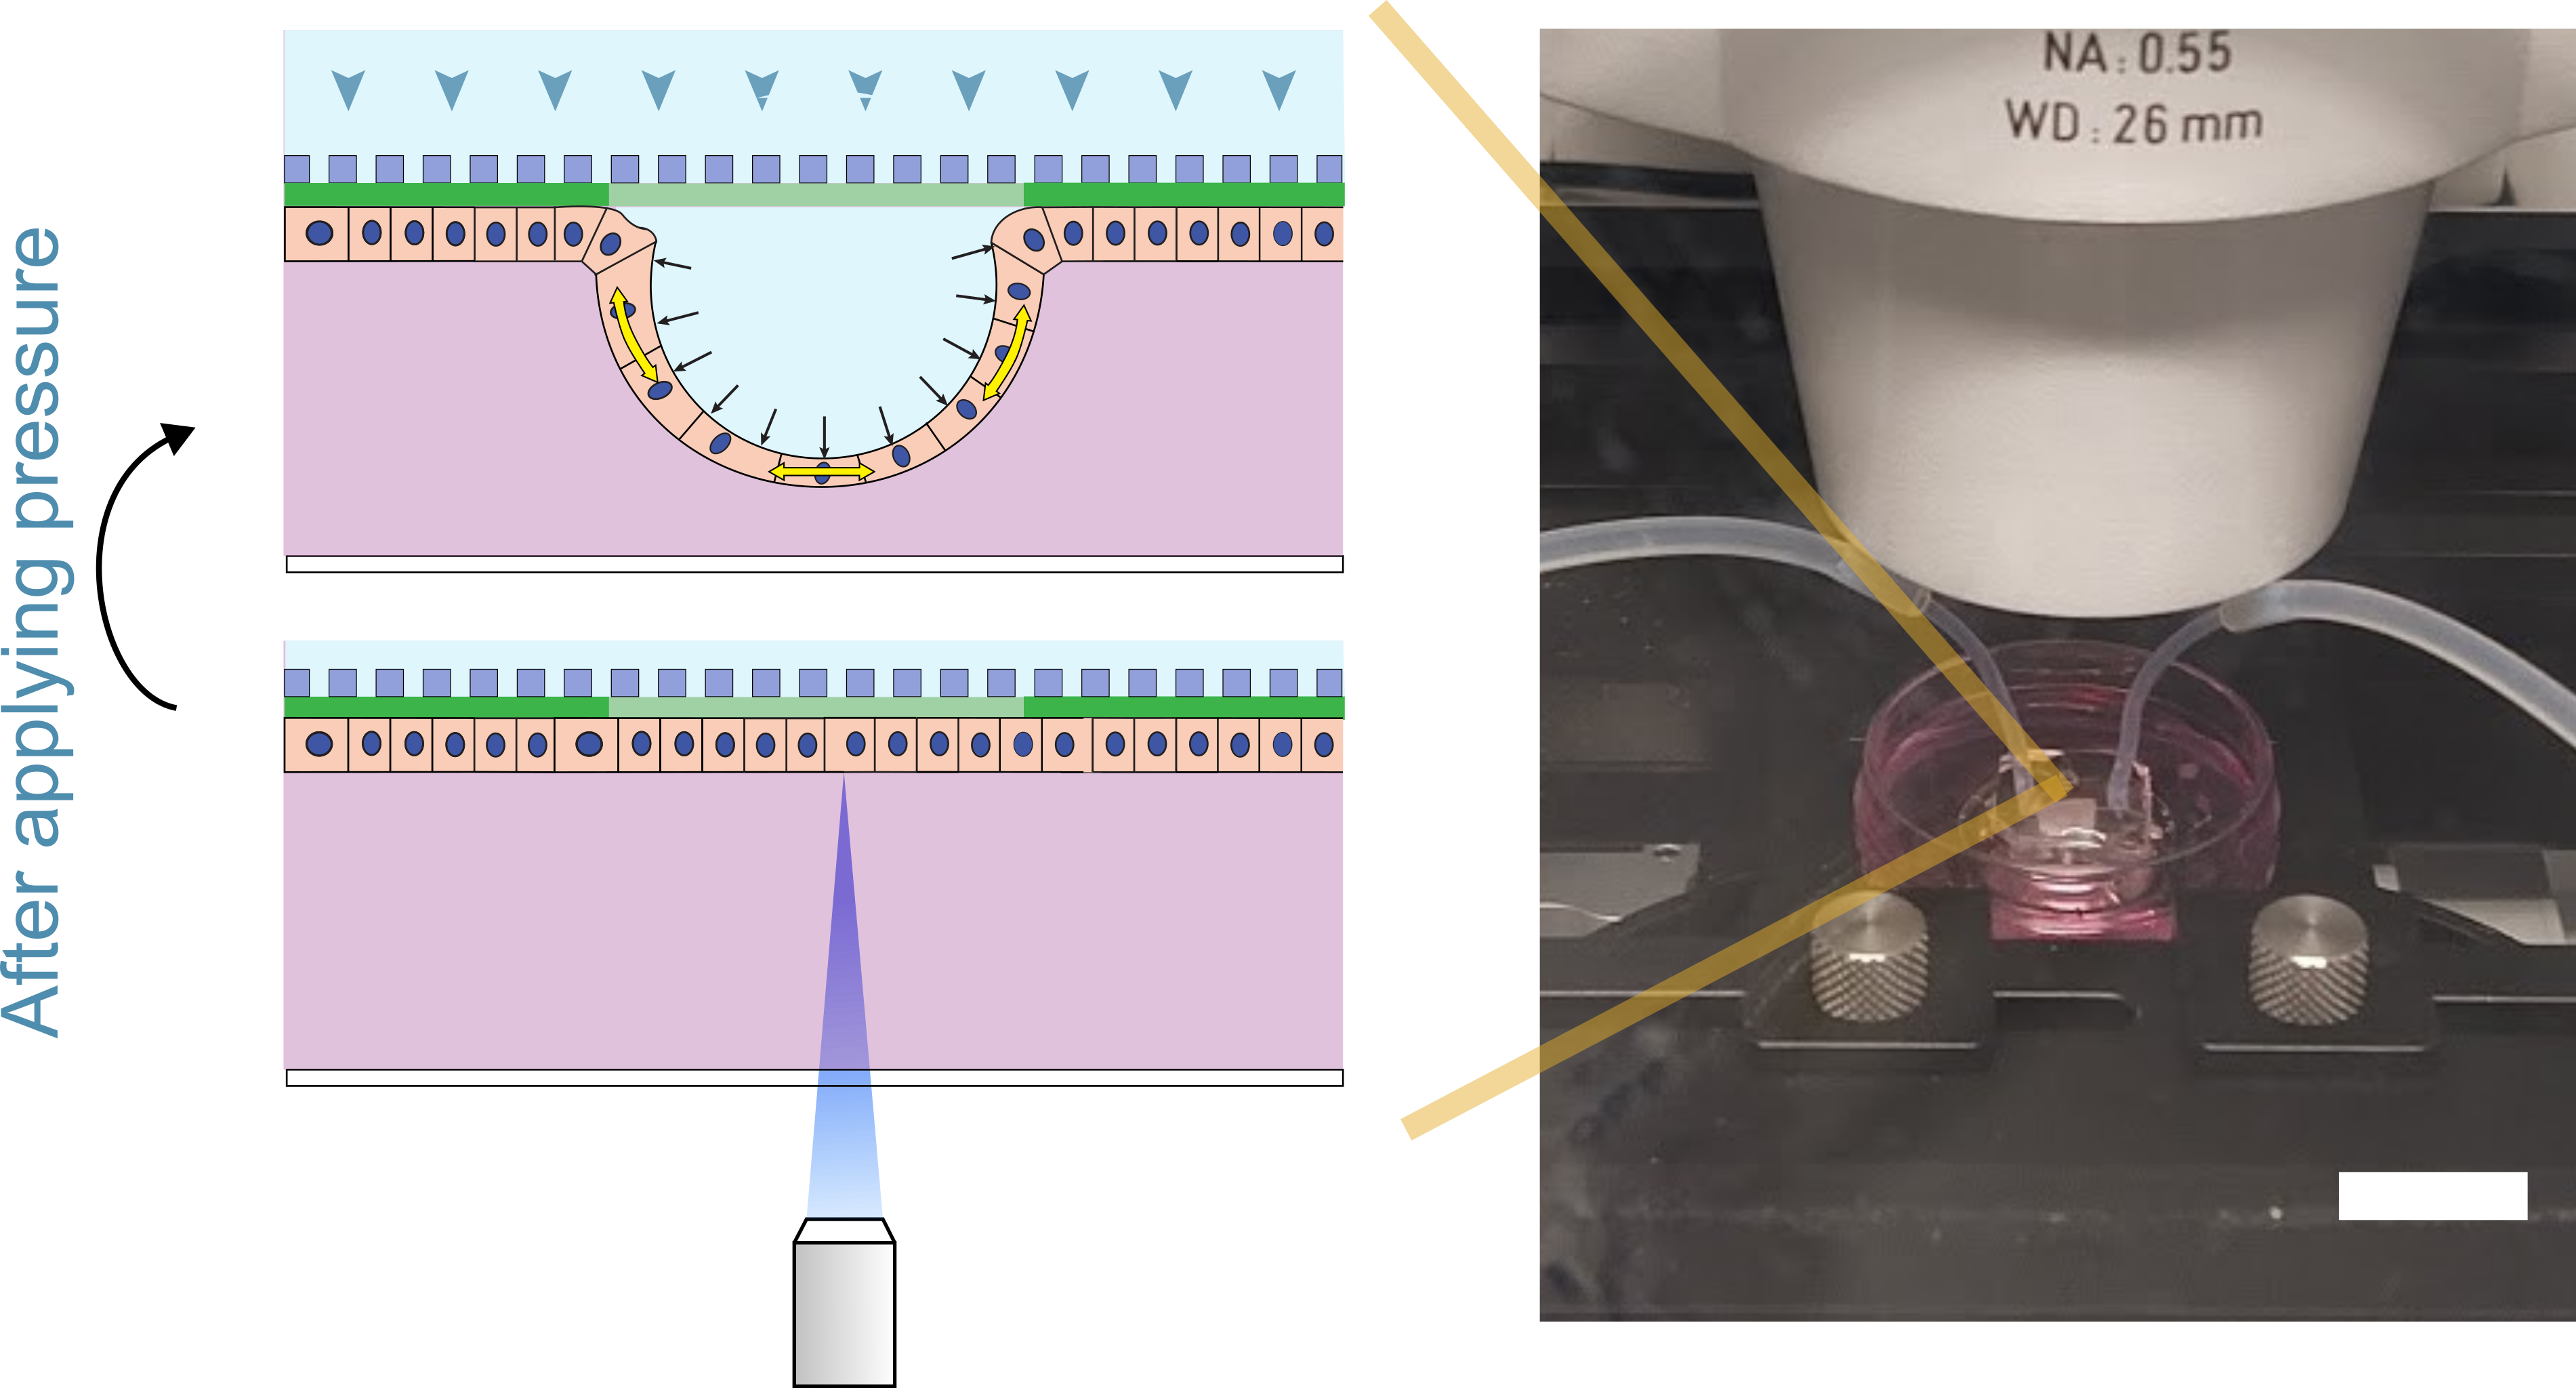
\includegraphics[width=0.75\textwidth]{chap6_realdevice.png}
	\caption{\textbf{Upside-down cell culture}: Illustration of upside-down cell culture and the experimental setup on the microscope stage.}\label{fig_6_5}
\end{figure}

\hypertarget{pressure-control}{%
\section{Pressure control}\label{pressure-control}}

For the application of external pressure, we selected hydrostatic pressure as the method of choice. Previous studies had reported a pressure requirement of approximately 100 \unit{\pascal}, equivalent to 1 \unit{\cm} of water column, for the formation of a dome. Initially, pipette tips were employed to apply pressure, but we observed that they were susceptible to bubble formation and leaks. Hence, we switched to using Polytetrafluoroethylene tubing, which was connected to a 50 \unit{\ml} reservoir (Falcon tube) to mitigate these issues (see Fig. \ref{fig_6_3}). By adjusting the height of the tube to match the air-liquid interface in the reservoir with the device, zero pressure was exerted on the cell monolayer. To apply pressure, we increased the height of the tube by 2\unit{\cm}, resulting in the application of 200 \unit{\pascal} pressure to the monolayer, leading to the delamination of cells and the formation of domes.

Nonetheless, we exercised caution regarding the potential occurrence of bubble formation within the cell channel. To avoid this we subjected the media to a vacuum chamber for 30 \unit{\minute} prior to the experiment to eliminate any nascent bubbles that may have developed over time. During tubing insertion, however, the system posed a risk of reintroducing bubbles into the system. To counter this issue, we employed the two inlets for each channel to flush fresh media from the reservoir, ensuring that no bubbles were present.

\begin{figure}[h!]
	\centering
	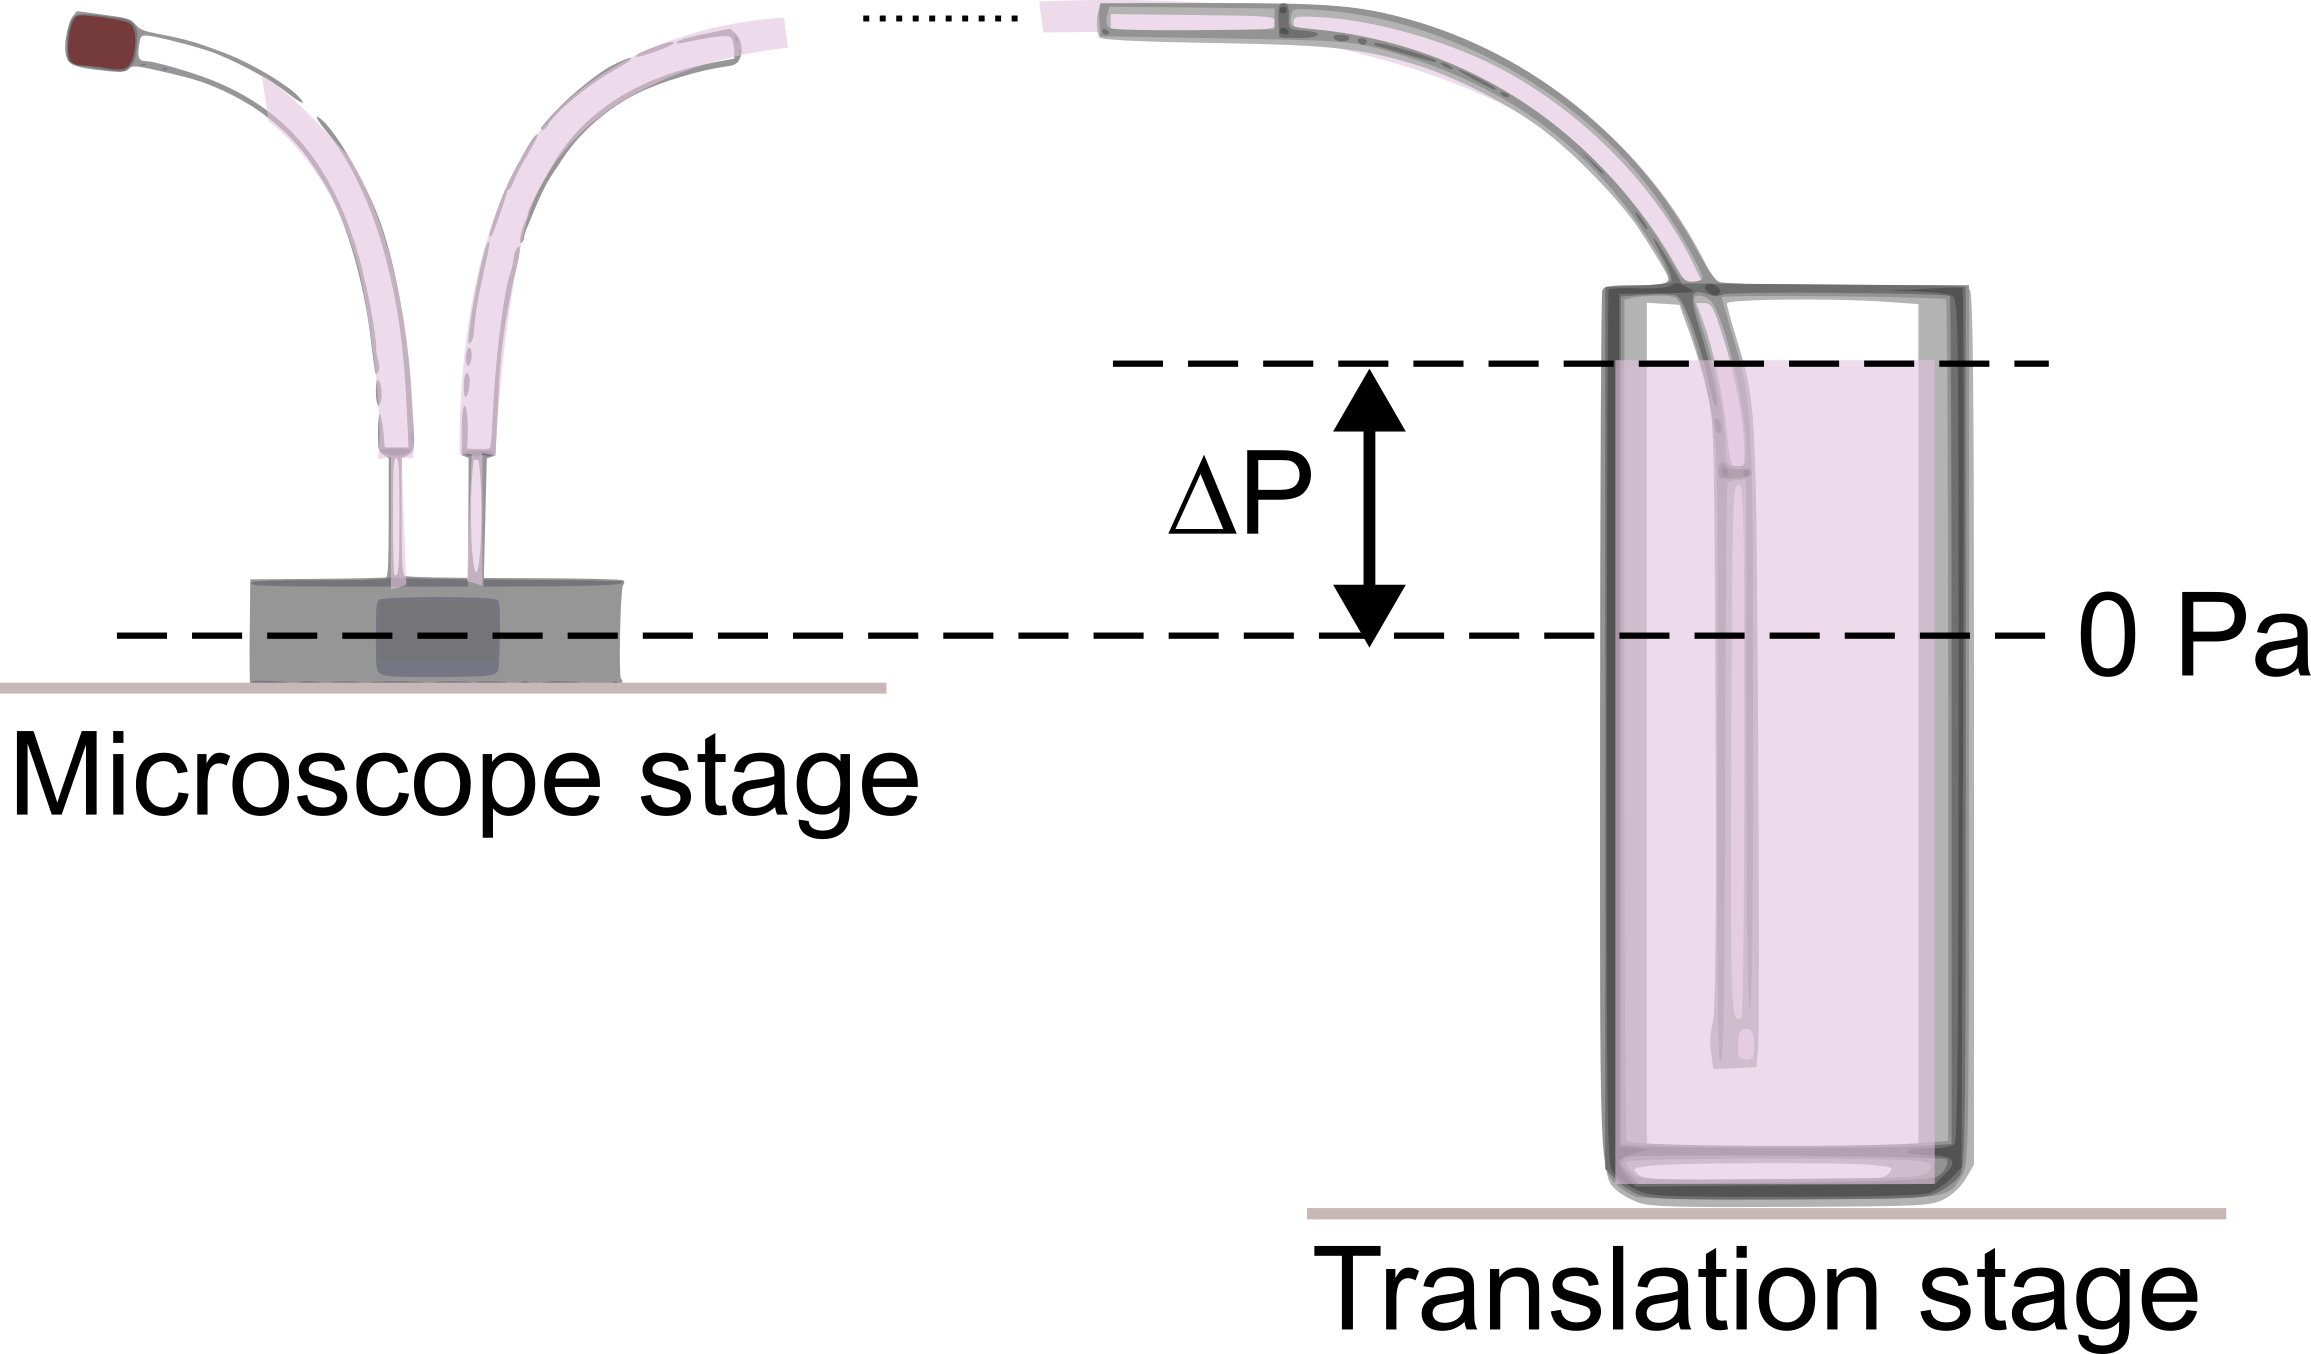
\includegraphics[width=0.65\textwidth]{chap6_pressure.png}
	\caption{\textbf{Hydrostatic pressure application}: The device is positioned on a microscope stage and connected to a reservoir of media, which in turn is attached to a translation stage. By increasing the difference between the device and the air-liquid interface, we can measure and apply hydrostatic pressure.	} \label{fig_6_3}
\end{figure}

To control the pressure, we used an automatic translation stage (Zaber High speed motorized linear stage) that could be programmed to lift the reservoir. We measured the pressure by tracking the height of the stage and the zero-pressure position. With this stage, we could apply pressure in the range of 0 $\rightarrow$ 1500 \unit{\pascal}, and we could even apply negative pressure by setting it lower. For our experiments, we used the range of -200 $\rightarrow$ 1300 \unit{\pascal}.

This translation stage is capable of accommodating linear velocities ranging from 0.000303 to 280 \unit{mm/s}, which correspond to pressure rates of 0.00303 to 2800 \unit{Pa/s}. At higher pressure rates, one may inquire about pressure losses within the device. To calculate these losses, we assumed that the walls of the microfluidic device remain undeformed given the small pressure differentials (200~Pa), and that all flow rate is due to changes in volume in the domes. Consider, an 80 \unit{\um} diameter dome with 100\% strain holds around 0.1 \unit{\ul} of fluid, which flows through a 5020 \unit{\micro\meter\squared} dome footprint. The membrane vendor specifies a limiting flow rate of 45~\unit{mL/min/cm^2} for water at 70~kPa. Assuming a linear relationship between flow rate and pressure, we can find that the flow rate through the dome footprint for a pressure of 200Pa to be 1.0952~$\times 10^{-13}$ \unit{\cubic\meter\per\second}. By considering the length of the tube (30~cm), its internal diameter (1~mm), and the dynamic viscosity of water (1~mPas), we can use the Poiseuille equation to estimate the pressure loss in the tubes to be 0.4523 Pa. This value is negligible in comparison to the pressures that are applied in the system.

%\begin{figure}
%	\begin{minipage}[c]{0.6\textwidth}
%		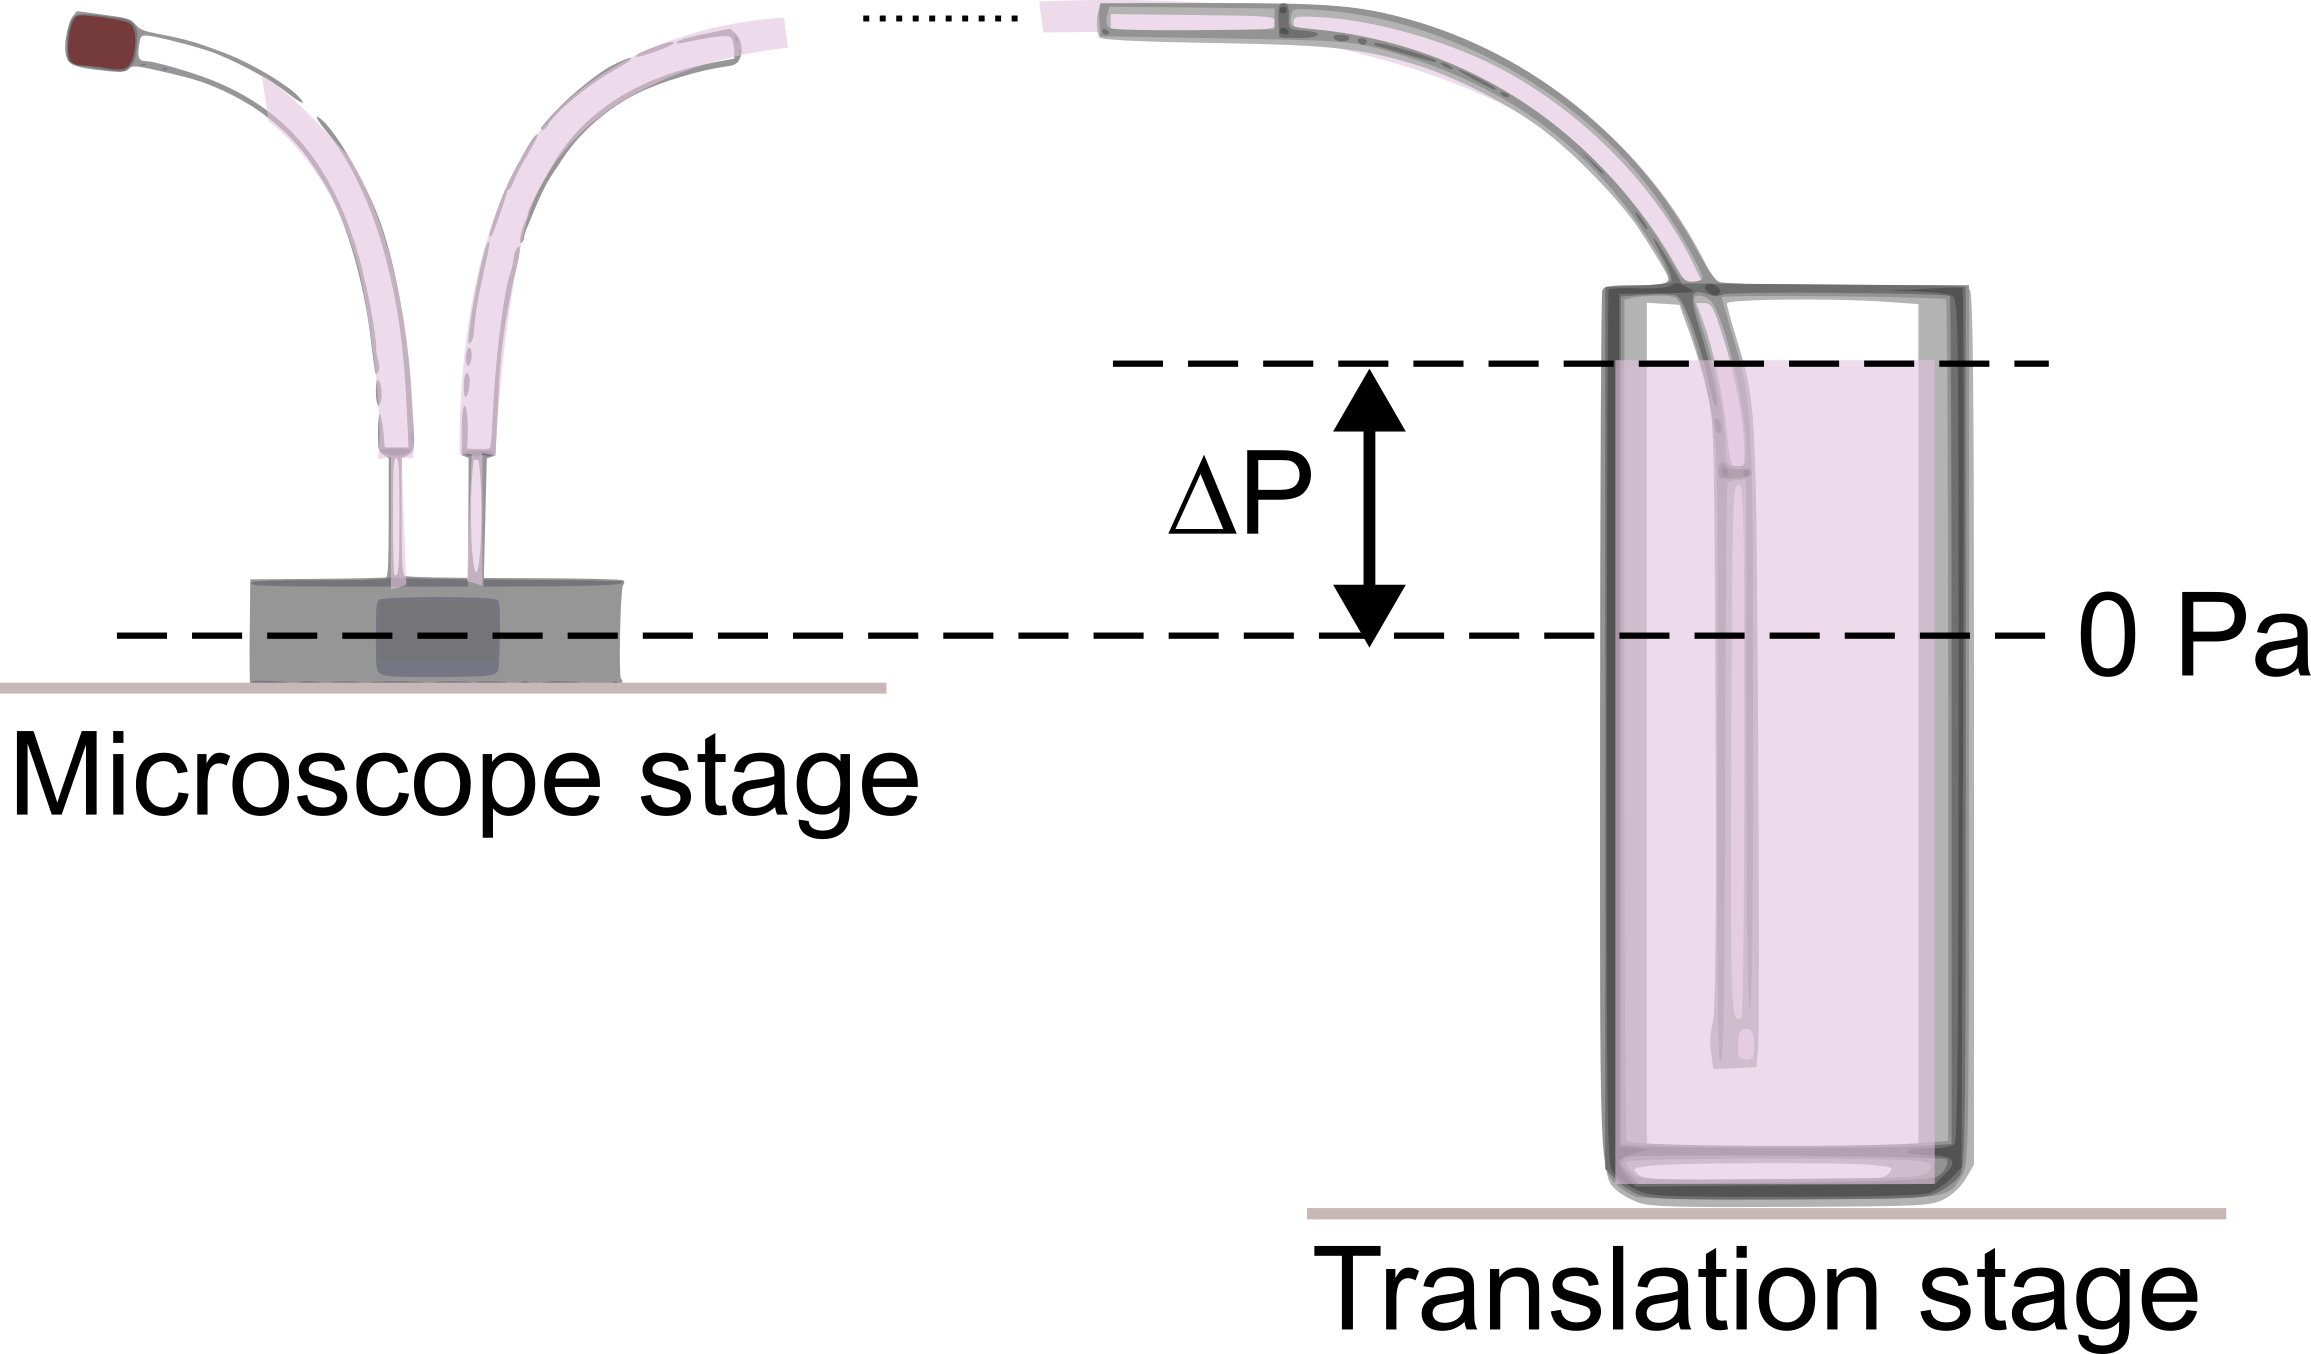
\includegraphics[width=\textwidth]{chap6_pressure.png}
%	\end{minipage}\hfill
%	\begin{minipage}[c]{0.35\textwidth}
%		\caption{\\ \textbf{Hydrostatic pressure application}:\\ The device is positioned on a microscope stage and connected to a reservoir of media, which in turn is attached to a translation stage. By increasing the difference between the device and the air-liquid interface, we can measure and apply hydrostatic pressure.
%		} \label{fig_6_3}
%	\end{minipage}
%\end{figure}

\hypertarget{imaging-the-epithelial-domes}{%
\section{Imaging the epithelial
domes}\label{imaging-the-epithelial-domes}}

Following extensive optimization of protein patterning, cell culture conditions, and confocal microscopy techniques, we were able to generate domes in accordance with the intended pattern and exert precise control over the pressure required for their formation. To obtain images of the dome, we utilized a spinning disk confocal microscope with a 40x objective lens (NA 0.75), which allowed us to visualize the membrane (CIBN CAAX GFP) and adhesion protein (Fibrinogen) pattern in separate channels (488\unit{\nm} and 644\unit{\nm}, respectively). By incorporating a labeled adhesion protein, we were able to track the formation of the domes with greater ease and accuracy.

\begin{figure}[h!]
	\centering
	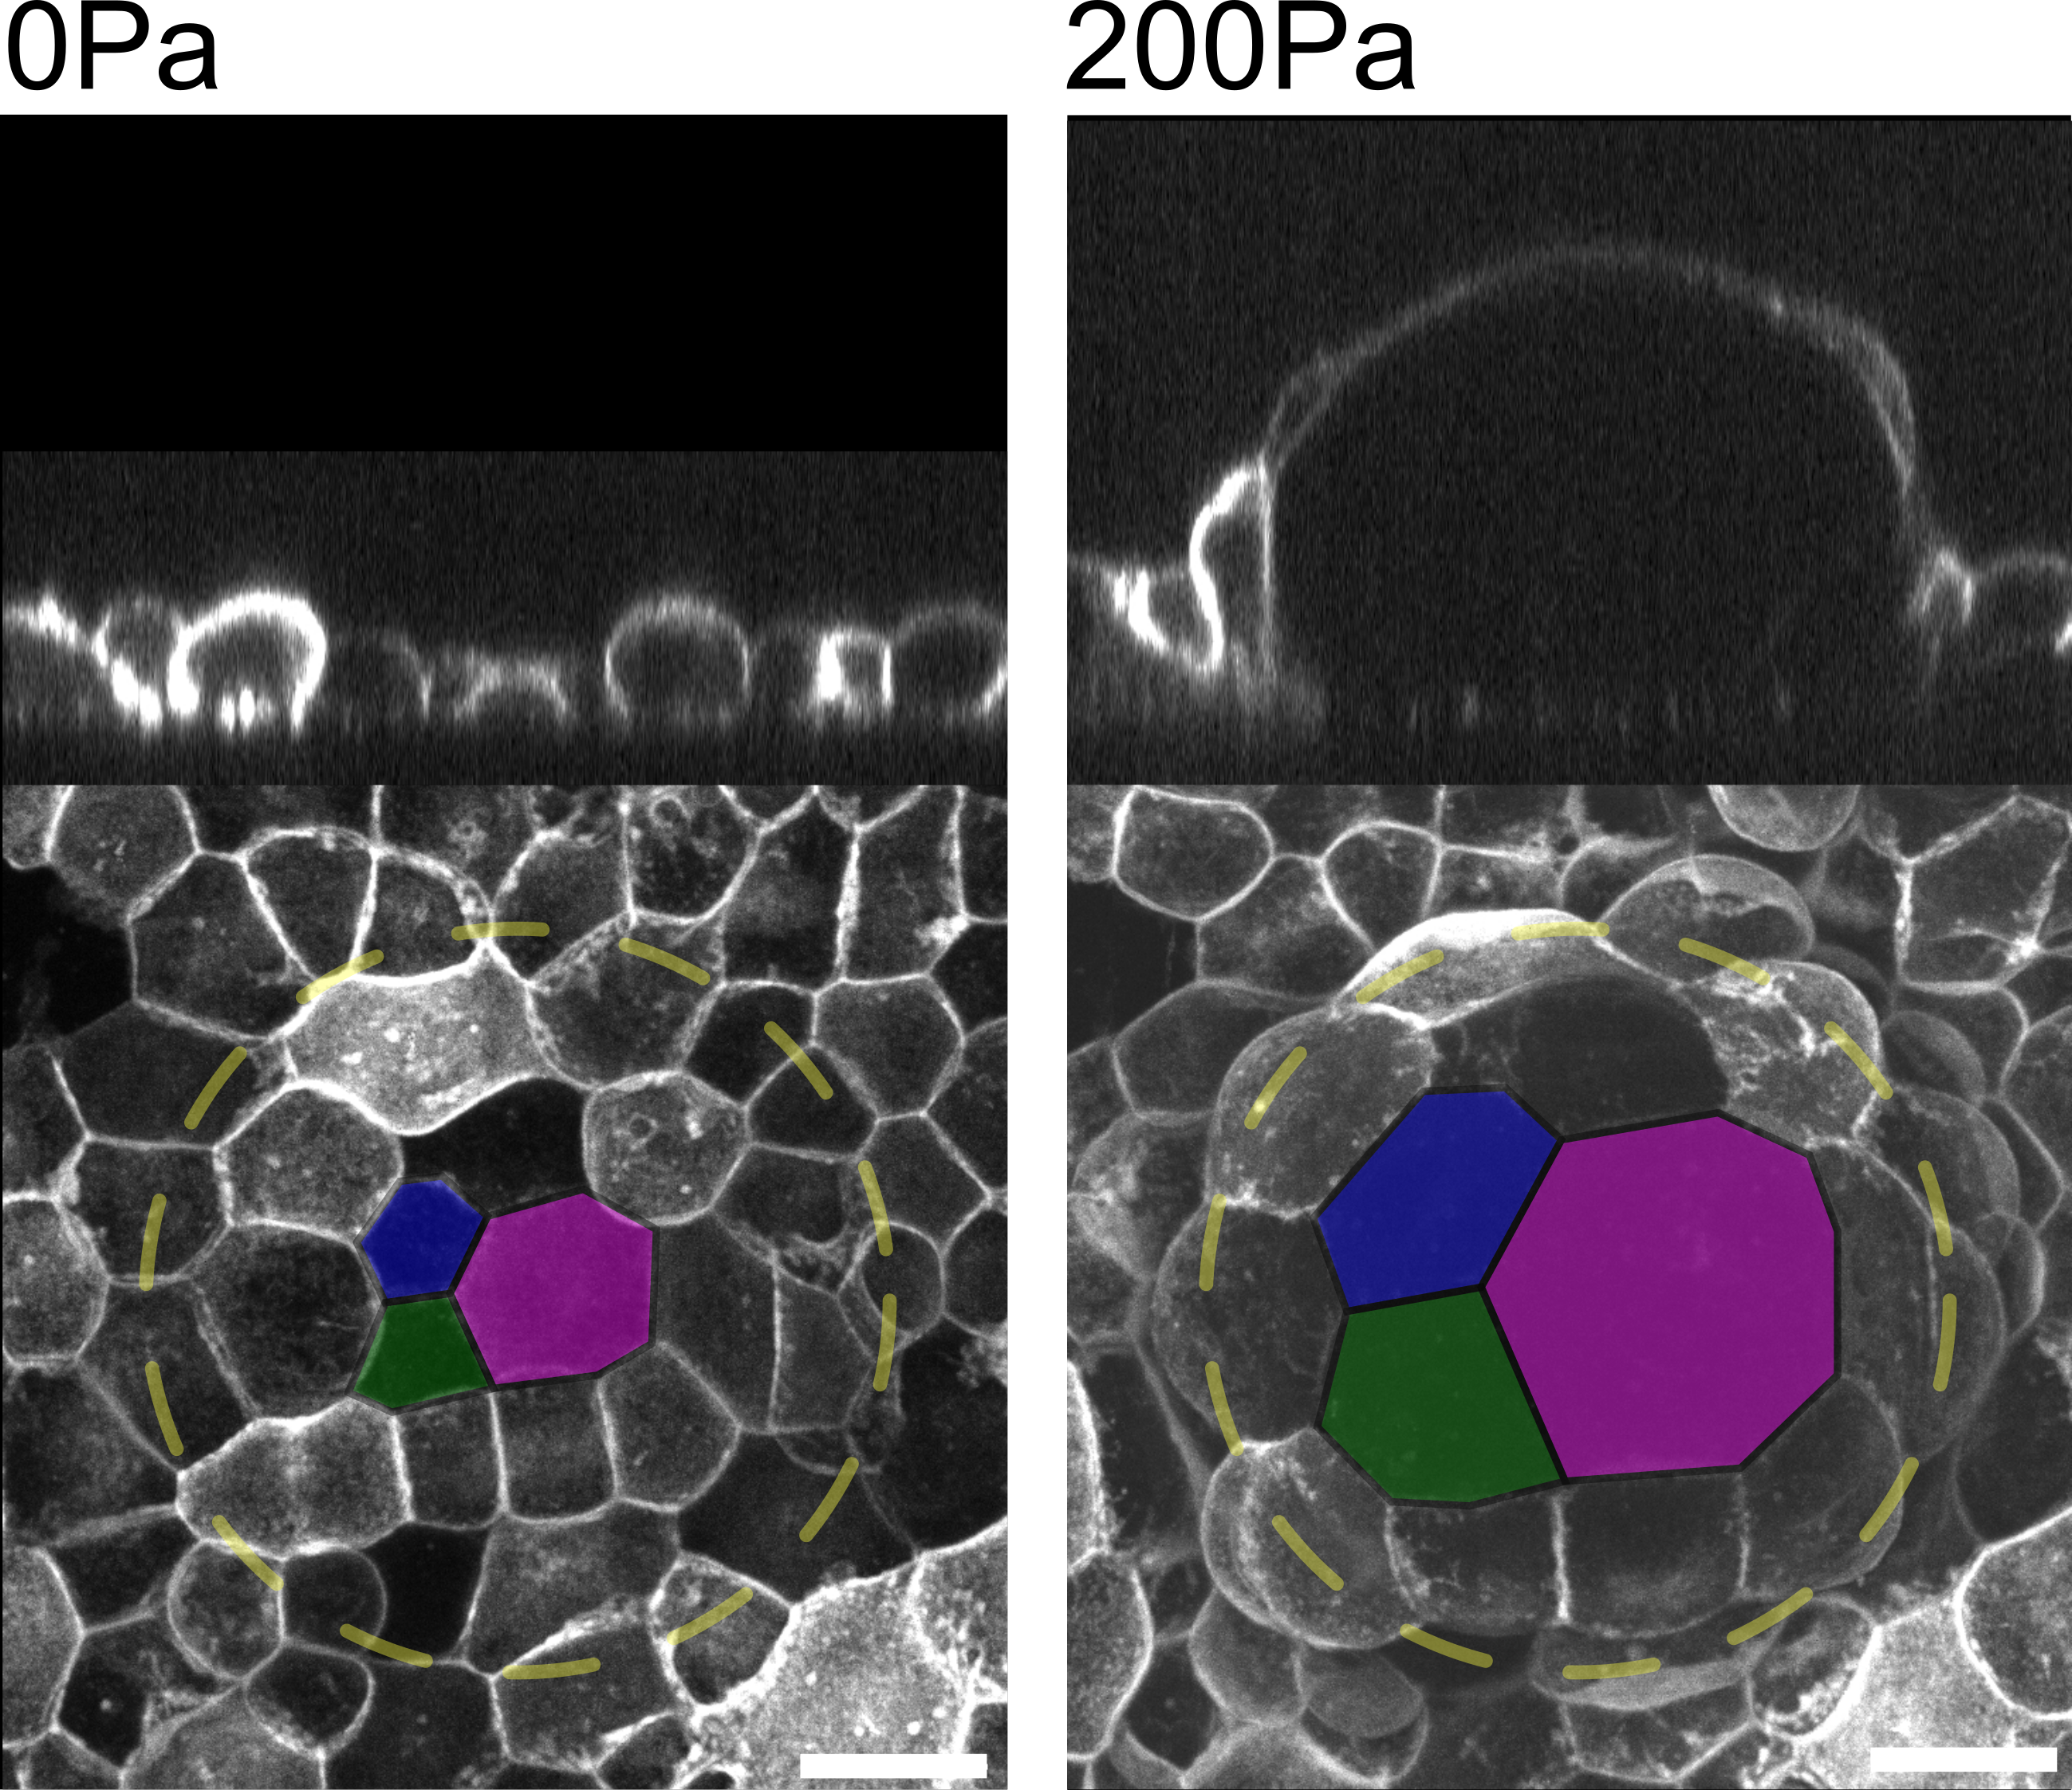
\includegraphics[width=0.7\textwidth]{chap6_confocaldomes.png}
	\caption{\textbf{Epithelial dome:} Representative confocal microscopy sections of domes at 0 Pa and 200 Pa. Images in the XY plane represent the dome's maximum projection, while images in the XZ plane represent a cross section at the center plane. Three cells are highlighted with color to show the stretching during the dome inflation. Scale bar is $20 \mu m$.
	} \label{fig_6_6}
\end{figure}
\clearpage

We initially focused on characterizing the mechanics of spherical domes at constant pressure to gain insights into epithelial behavior (see Fig. \ref{fig_6_6}). Laplace's law was employed to calculate tension using pressure, cell shape, and tissue curvature data, which we could easily monitor. Unlike previous studies that did not control the pressure under the dome, our experimental system allowed us to inflate and deflate the domes in seconds. This forced us to monitor them by observing the base of the dome where the monolayer would intermittently come in and out of view.

Acquiring images of the dome stack in a confocal microscope required three minutes using a step size of 0.5\unit{\um} (exposure 500\unit{\ms}) and a height of 100\unit{\um}, which was slower than the rate at which we could deform the dome by changing the pressure (see Fig. \ref{fig_6_6}). To investigate the rheology of the domes, it was necessary to monitor their dynamic response at faster pressure rates and shorter timescales while measuring dome strain and curvature. Since the dome possessed inherent symmetry, imaging the mid-section of the structure provided all the geometric information required.

\begin{figure}[h!]
	\begin{minipage}[c]{0.6\textwidth}
		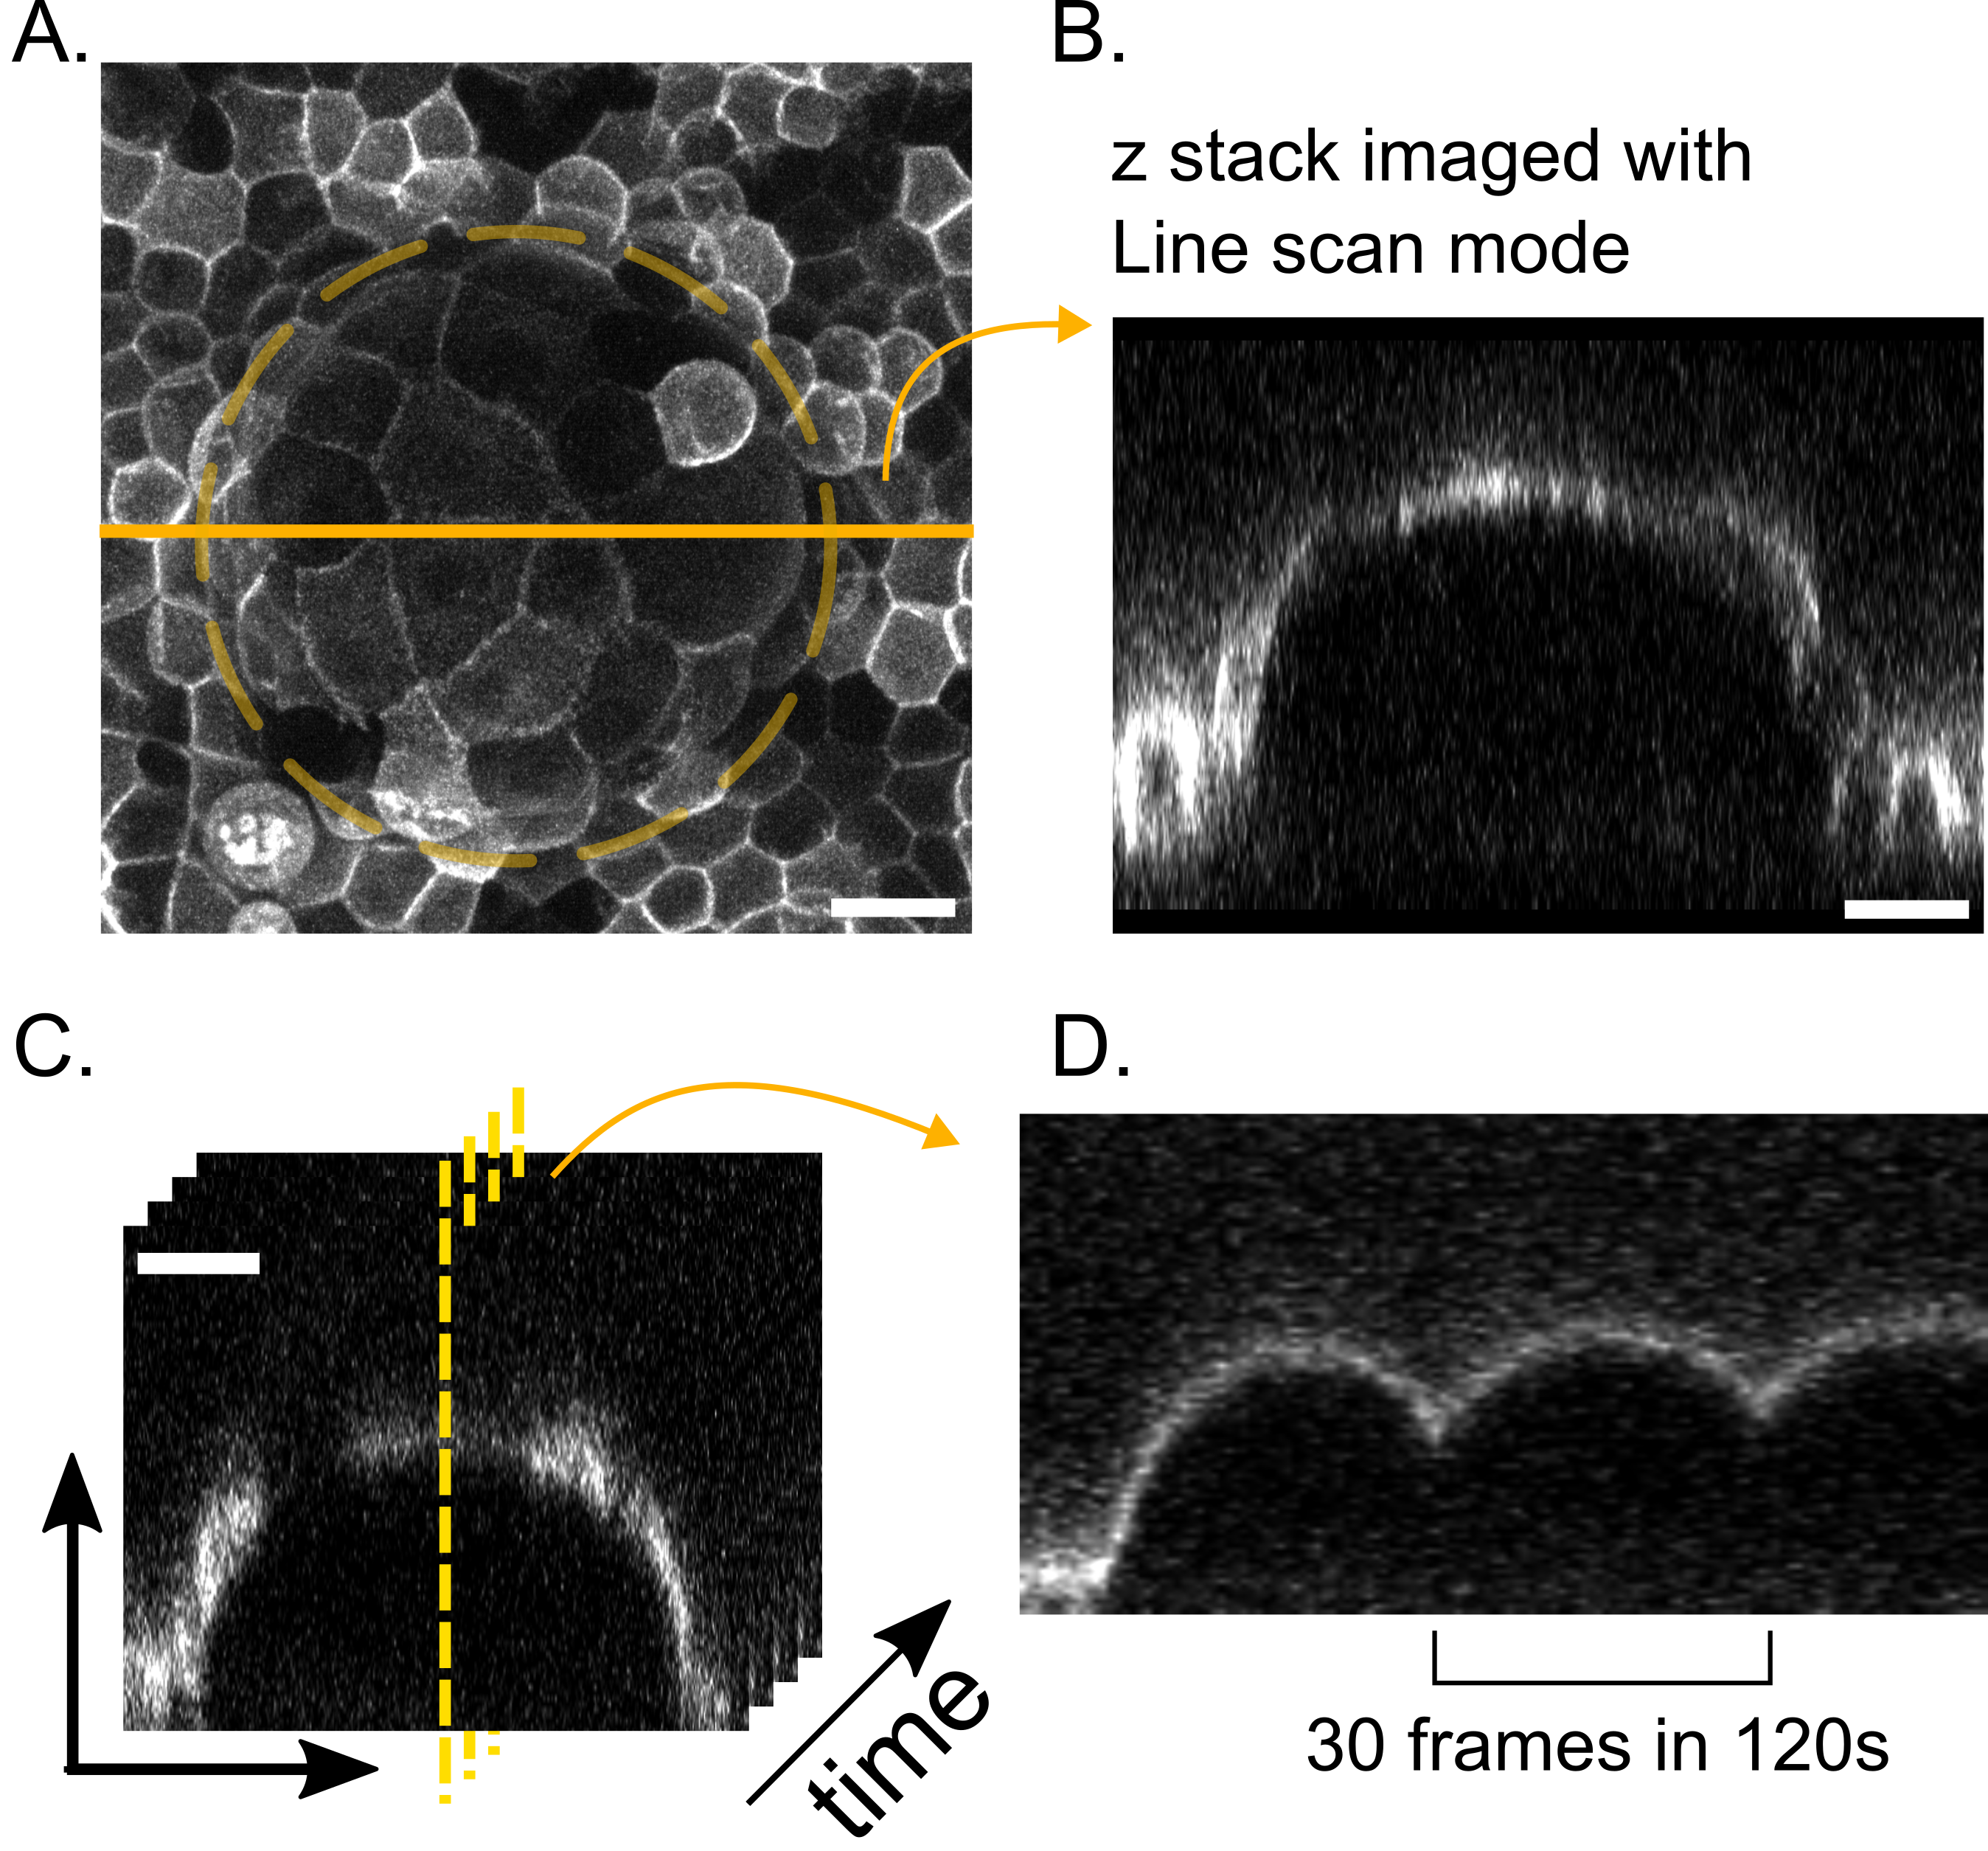
\includegraphics[width=\textwidth]{chap6_LSM.png}
	\end{minipage}\hfill
	\begin{minipage}[c]{0.35\textwidth}
		\caption{\\ \textbf{Imaging the dome with Line scanning mode:}\\ (A) Confocal microscopy image of a dome's maximum projection. (B) Midsection of the same dome imaged with the line scan mode (LSM). (C-D) Timelapse of the dome in LSM and a kymograph showing dynamics of the domes when imaged at time-step of $4s$. Scale bars are $20 \mu m$.
		} \label{fig_6_7}
	\end{minipage}
\end{figure}

Using the line scanning mode of a Zeiss Airy Scan Microscope, we imaged a single line of pixels across the midsection of the dome and acquired a confocal z-stack (1024 pixel, 4.1\unit{\us/pixel} dwell time, and 1\unit{\um} step size) along the height of the dome (refer to Fig. \ref{fig_6_7}). This approach allowed us to obtain a cross-sectional view of the dome in a fraction of the time required for a normal stack. By enabling piezo stage movement, we imaged a 100\unit{\um} tall dome in just 4 seconds and tracked its height evolution using a kymograph of the central part of the dome. It is important to note that this imaging method is primarily useful for tracking dome strain and curvature, and the cell images obtained are often of low quality.


\hypertarget{light-sheet-moli}{%
\section{Light-sheet MOLI}\label{light-sheet-moli}}

We utilized a Brucker QuVi SPIM light sheet microscope to capture rapid subcellular or cellular changes. The microscope was equipped with two immersion-upright 40x objectives (NA 0.8) at 45\unit{\degree} to the horizontal plane. Drawing upon our proficiency in device fabrication, we devised a new setup that facilitated top imaging of cells and porous membranes (see Fig. \ref{fig_6_8}).

\begin{figure}[h!]
	\centering
	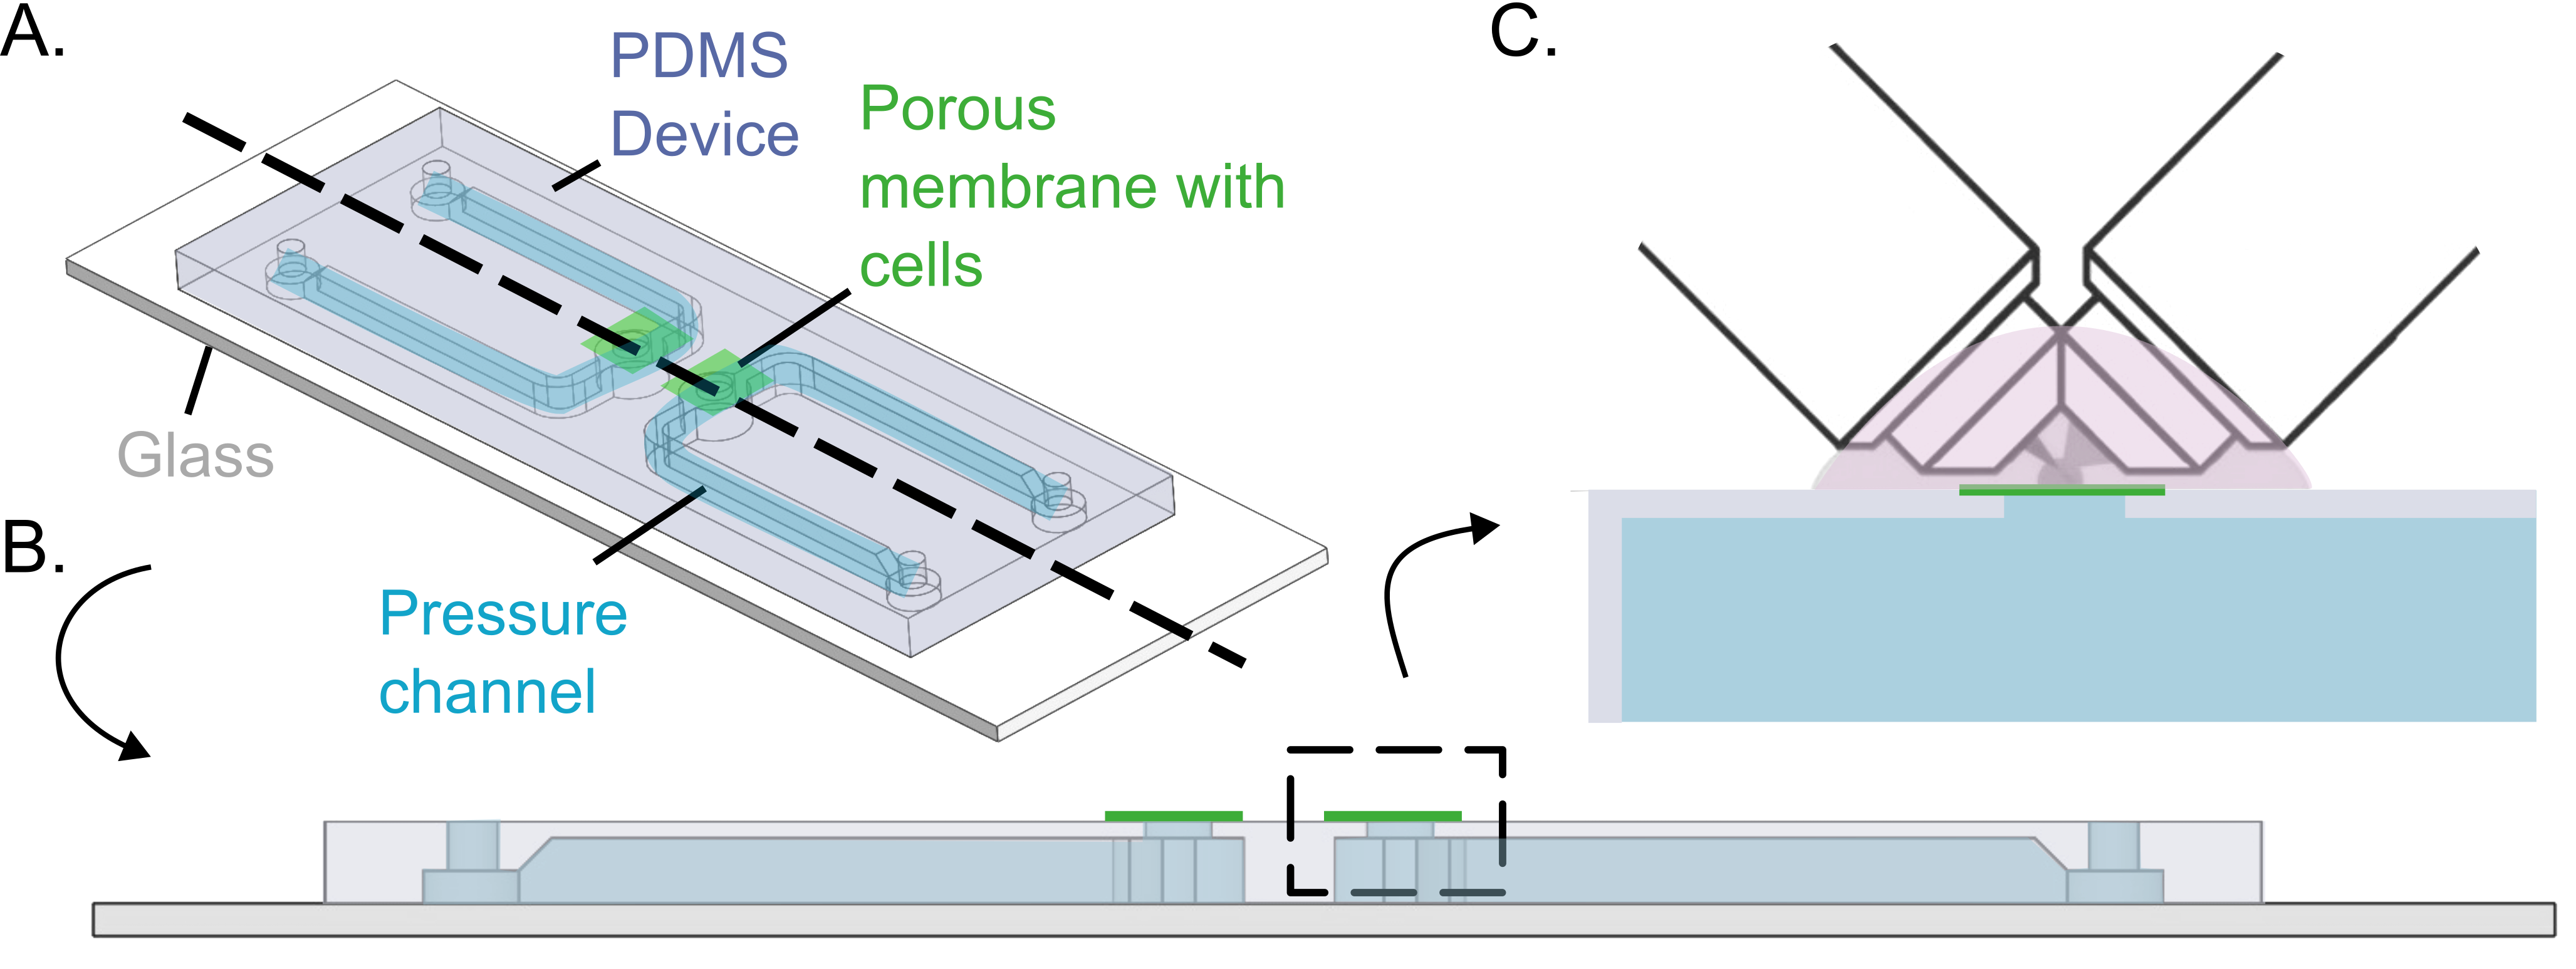
\includegraphics[width=\textwidth]{chap6_lightsheet.png}
	\caption{ \textbf{Light sheet MOLI}: (A) Isometric illustration of a single piece PDMS block engraved with two channels, so that we can have two devices in one. (B) Cross-section of the device. (C) The device is used with 40x immersion objectives coming at $45 \deg$ angle. This limits to the field of view to $332\times 332\mu m^2$.
	}\label{fig_6_8}
\end{figure}

To simplify the fabrication process, we inverted the conventional MOLI device. This necessitated only a pressure channel and a middle layer with a hole and porous membrane. The device was manufactured sufficiently thick to plug in the tubing, and given the device and channels' size, we produced the mold using a standard 3D printer, Ultimaker 3D printer. We incorporated a ridge-like protrusion to manufacture the pressure channel and cell seeding hole in one go. The device was bonded to a microscope slide using unpolymerized PDMS, and we performed PRIMO patterning of the device by flipping it upside down. In this setup, seeding cells was easier, as the cell seeding part was exposed.

As expected, we were able to generate domes using the same system as before by applying pressure. The imaging technique we developed enabled us to acquire a full dome image in a mere 4 seconds, which involves using objective scan, where only one objective to scan the dome with 100 frames with step size of 1\unit{\um} at rate of 4\unit{\ms}. This allows us to observe fast-moving features that were indiscernible with other imaging techniques (see Fig. \ref{fig_6_9}).

\begin{figure}[]
	\centering
	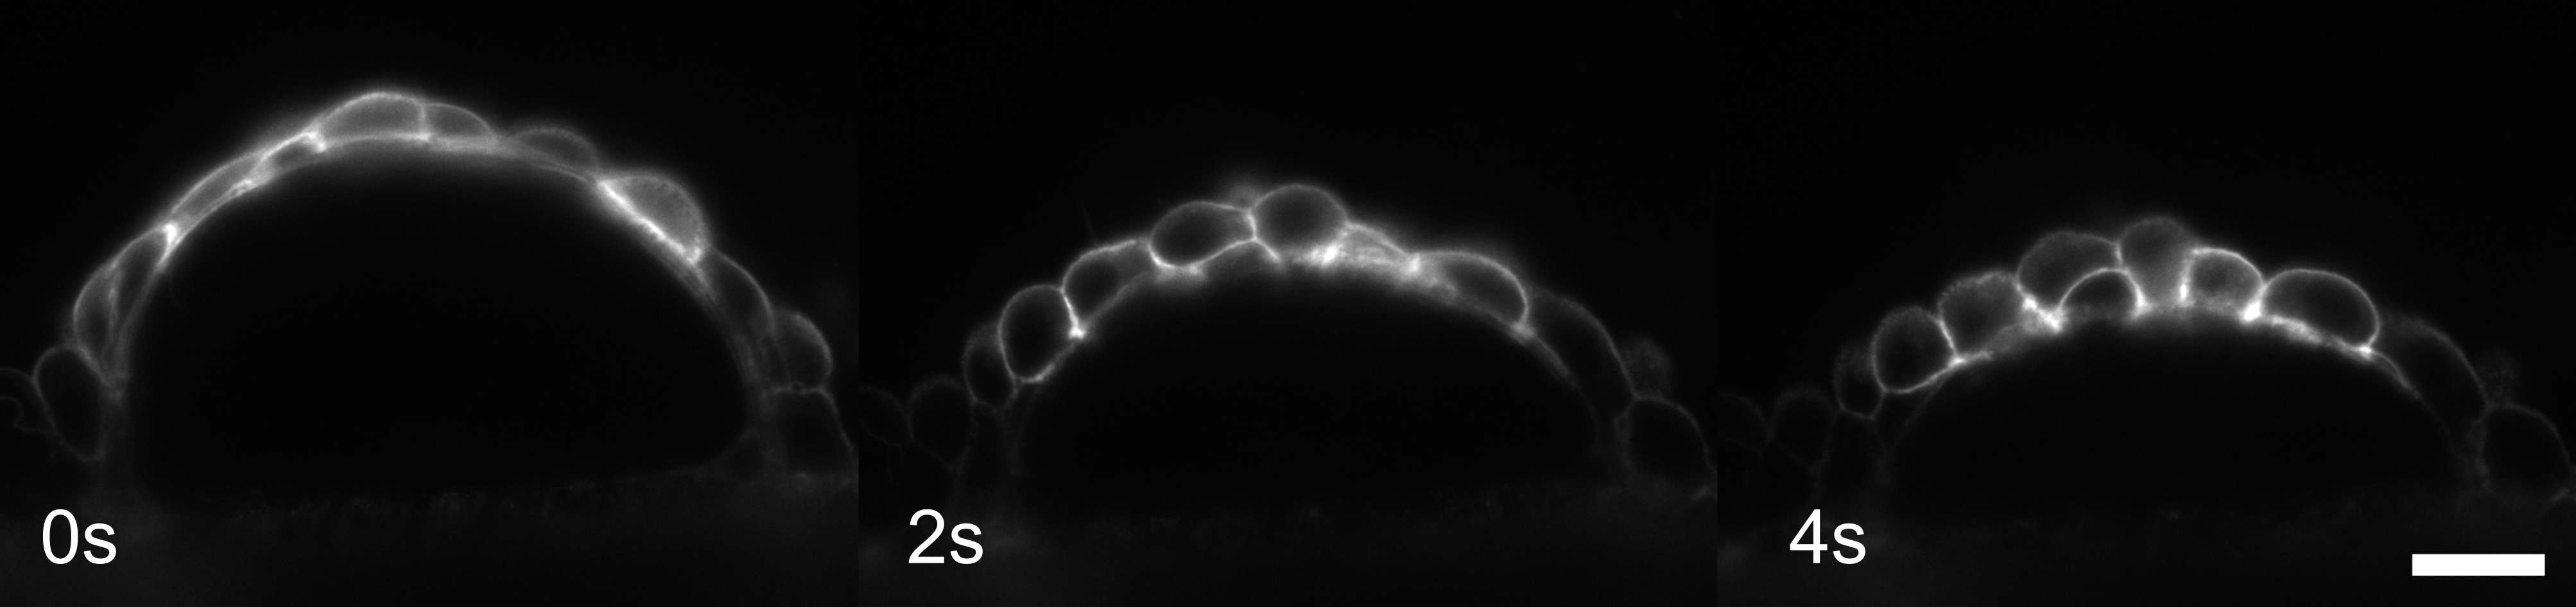
\includegraphics[width=0.8\textwidth]{chap6_lightsheetdome.png}
	\caption{ \textbf{Dome imaged with Light sheet MOLI}: Mid-section of a dome with membrane marker imaged every $2s$. Showing the shape of individual cells undergoing changes during deflation. Scale bar is $20 \mu m$.
	}\label{fig_6_9}
\end{figure}

\hypertarget{summary-and-discussion}{%
\section{Summary and Discussion}\label{summary-and-discussion}}

We have developed a microfluidic chip to generate 3D curved epithelia, utilizing a multilevel device consisting of two layers separated by a porous membrane. Seeding cells on the membrane in the bottom channel allowed for dome formation closer to the microscope objective, enabling high-quality confocal imaging. Hydrostatic pressure was under the dome was controlled dynamically, allowing for monitoring of cells and tissue behavior. Additionally, we developed imaging strategies to capture dynamics of these 3D structures faster using line scanning mode of confocal microscope or light sheet microscope.

Using this device, we were able to form the domes and monitor cellular and tissue behavior. As demonstrated in previous studies, the most intriguing aspect of the system is that complex materials such as epithelial tissue, in order to maintain mechanical equilibrium, must adopt a spherical cap shape for a circular footprint. This uniform curvature and pressure imply uniform and isotropic tension, independent of tissue material properties \cite{latorre2018,marin-llaurado2022}. The tissue tension can be easily measured by applying Laplace's law for spherical cap domes. However, in the case of non-spherical geometry, there would be anisotropic stresses that would require a computational model, such as curved monolayer stress microscopy, to solve an inverse problem to go from geometry to forces \cite{marin-llaurado2022}.  

The geometry of the domes is primarily controlled by the adhesion protein pattern, but delamination can still occur. In spontaneous domes, circular footprints were found to be the most common  \cite{tanner1983}, while domes formed around sharp corners can blunt themselves through delamination \cite{latorre2018}. This must be taken into consideration when creating specific geometries. Tissue tension and adhesion forces also interact with each other. In MDCK suspended monolayer, it is seen that cell-cell junctions are stronger than cell-substrate adhesion \cite{harris2012}, so if tension at the base of the dome exceeds the adhesion forces, it can lead to detachment and delamination.  

Furthermore, although not studied systematically here, MOLI can be used as a quantitative peeling system to probe tissue detachment from the substrate. If the dome retains its spherical shape, we can calculate the forces required to break cell-substrate adhesion and identify the contribution of focal adhesion molecular components.

This system provides a novel approach for testing material properties and probing mechanics at the tissue scale, allowing for simultaneous high-quality imaging and monitoring of cytoskeletal components and the nucleus. Additionally, we can create a 3D tissue with controlled lumen pressure, providing a well-controlled protocol that is suitable for replicating curvature-pressure-tension conditions in various cell types, including those that do not actively pump ions and form spontaneous domes. However, our primary focus is on comprehending the mechanics of epithelial tissue under controlled pressure.